\documentclass[]{article}
\usepackage{amsmath}
\usepackage{amsfonts}
\usepackage{amssymb}
\usepackage{listings}
\usepackage{xcolor}
\usepackage{graphicx}
\usepackage{hyperref}
\usepackage{cancel}
\usepackage{algpseudocode}
\usepackage{capt-of}

\definecolor{codegreen}{rgb}{0,0.6,0}
\definecolor{codegray}{rgb}{0.5,0.5,0.5}
\definecolor{codepurple}{rgb}{0.58,0,0.82}
\definecolor{backcolour}{rgb}{0.95,0.95,0.92}

\lstdefinestyle{mystyle}{
	backgroundcolor=\color{backcolour},   
	commentstyle=\color{codegreen},
	keywordstyle=\color{magenta},
	numberstyle=\tiny\color{codegray},
	stringstyle=\color{codepurple},
	basicstyle=\ttfamily\footnotesize,
	breakatwhitespace=false,         
	breaklines=true,                 
	captionpos=b,                    
	keepspaces=true,                 
	numbers=left,                    
	numbersep=5pt,                  
	showspaces=false,                
	showstringspaces=false,
	showtabs=false,                  
	tabsize=2
}

\lstset{style=mystyle}
%opening
\title{CPSC532W Homework 4}
\author{Justin Reiher\\ Student ID: 37291151\\ CWL: reiher}
\date{}

\begin{document}

\maketitle

Link to public repository for homework 4:
\begin{center}
	\url{https://github.com/justinreiher/probProg_Fall2021/tree/main/CS532-HW4}
\end{center}

\section{Program 0: BBVI Implementation Details}
 Implementing algorithm 11 and 12 from the book are outlined as follows:
 For algorithm 11, the sample and observe functions,where a new variable $v$ is introduced which is the address to the node in question. If the node does not exist then it is added to the program environment variable $\sigma$. The implementation of the \texttt{sample} and \texttt{observe} case are as follows:
 \lstinputlisting[language = Python, linerange ={73-85}]{primitivesAD.py}
 Like in the textbook, the \texttt{sample} case computes the \texttt{gradLogProb} of the sample from \emph{Q}:
 \lstinputlisting[language = Python, linerange ={186-194}]{primitivesAD.py}
 Since we only want the gradient, a copy of the distribution object \texttt{Dobj} is made to then compute the \texttt{gradLogProb} and then subsequently the result is \texttt{detached}. If we do not do this, then the gradients are compounding and create an exponentially growing gradient compute tree.
 The BBVI algorithm is implemented as follows:
 \lstinputlisting[language = Python, linerange ={51-86}]{bbvi.py}
 A topological graph sort is performed on the nodes before hand and stored. The nodes are then initially populated and for every random variable with an associated $\mathcal{Q}(v)$ gets an optimization object initialized with the parameters of the prior associated with node $v$. The optimizer used in this case is \texttt{Adam}. This distribution object is used to make an update step, copy over the update to $\mathcal{Q}(v)$ and continue. The optimization requires computing the weighted gradients. The gradient keys are merged together because under differing control flow it's possible that some gradients don't exist in some traces. In these instances the gradients are computed to zero:
  \lstinputlisting[language = Python, linerange ={107-140}]{bbvi.py}
 and subtracting the \emph{baseline}. The \emph{baseline} is computed by computing the element-wise covariance of each mini-batch trace and the weighted gradients and then summed. Any results resulting in \emph{nan} are turned to zeros using \texttt{torch.nan\_to\_num}. Using \texttt{numpy} \texttt{cov} routine returns a \texttt{dtype=float64} result, this is truncated back to \texttt{torch.float32} (This baseline computation was discussed at length with many of my classmates)
  \lstinputlisting[language = Python, linerange ={142-167}]{bbvi.py}
 The optimization step retrieves the optimization object associated with the $\mathcal{Q}(v)$ that is being optimized, a step is taken the gradients are then set to zero (same reason as to why the log-weights are detached after being computed) and the distribution object in $\mathcal{Q}(v)$ is updated with the new parameters:
 \lstinputlisting[language = Python, linerange ={171-186}]{bbvi.py}
 Finally, the results of the samples, the log-weights are stored and then returned.
\subsection{Program 1}
Number of samples per optimization is: 200, number of optimization steps is: 350, Adam learning rate: 0.5
\begin{verbatim}
Collect samples denoted by program 1:
Elapsed time for program  1 .daphne is:  0:01:28.018433  seconds
Mean of set of samples:  tensor(7.2636) 
and variance of samples:  tensor(0.0539)	
\end{verbatim}
\begin{center}
	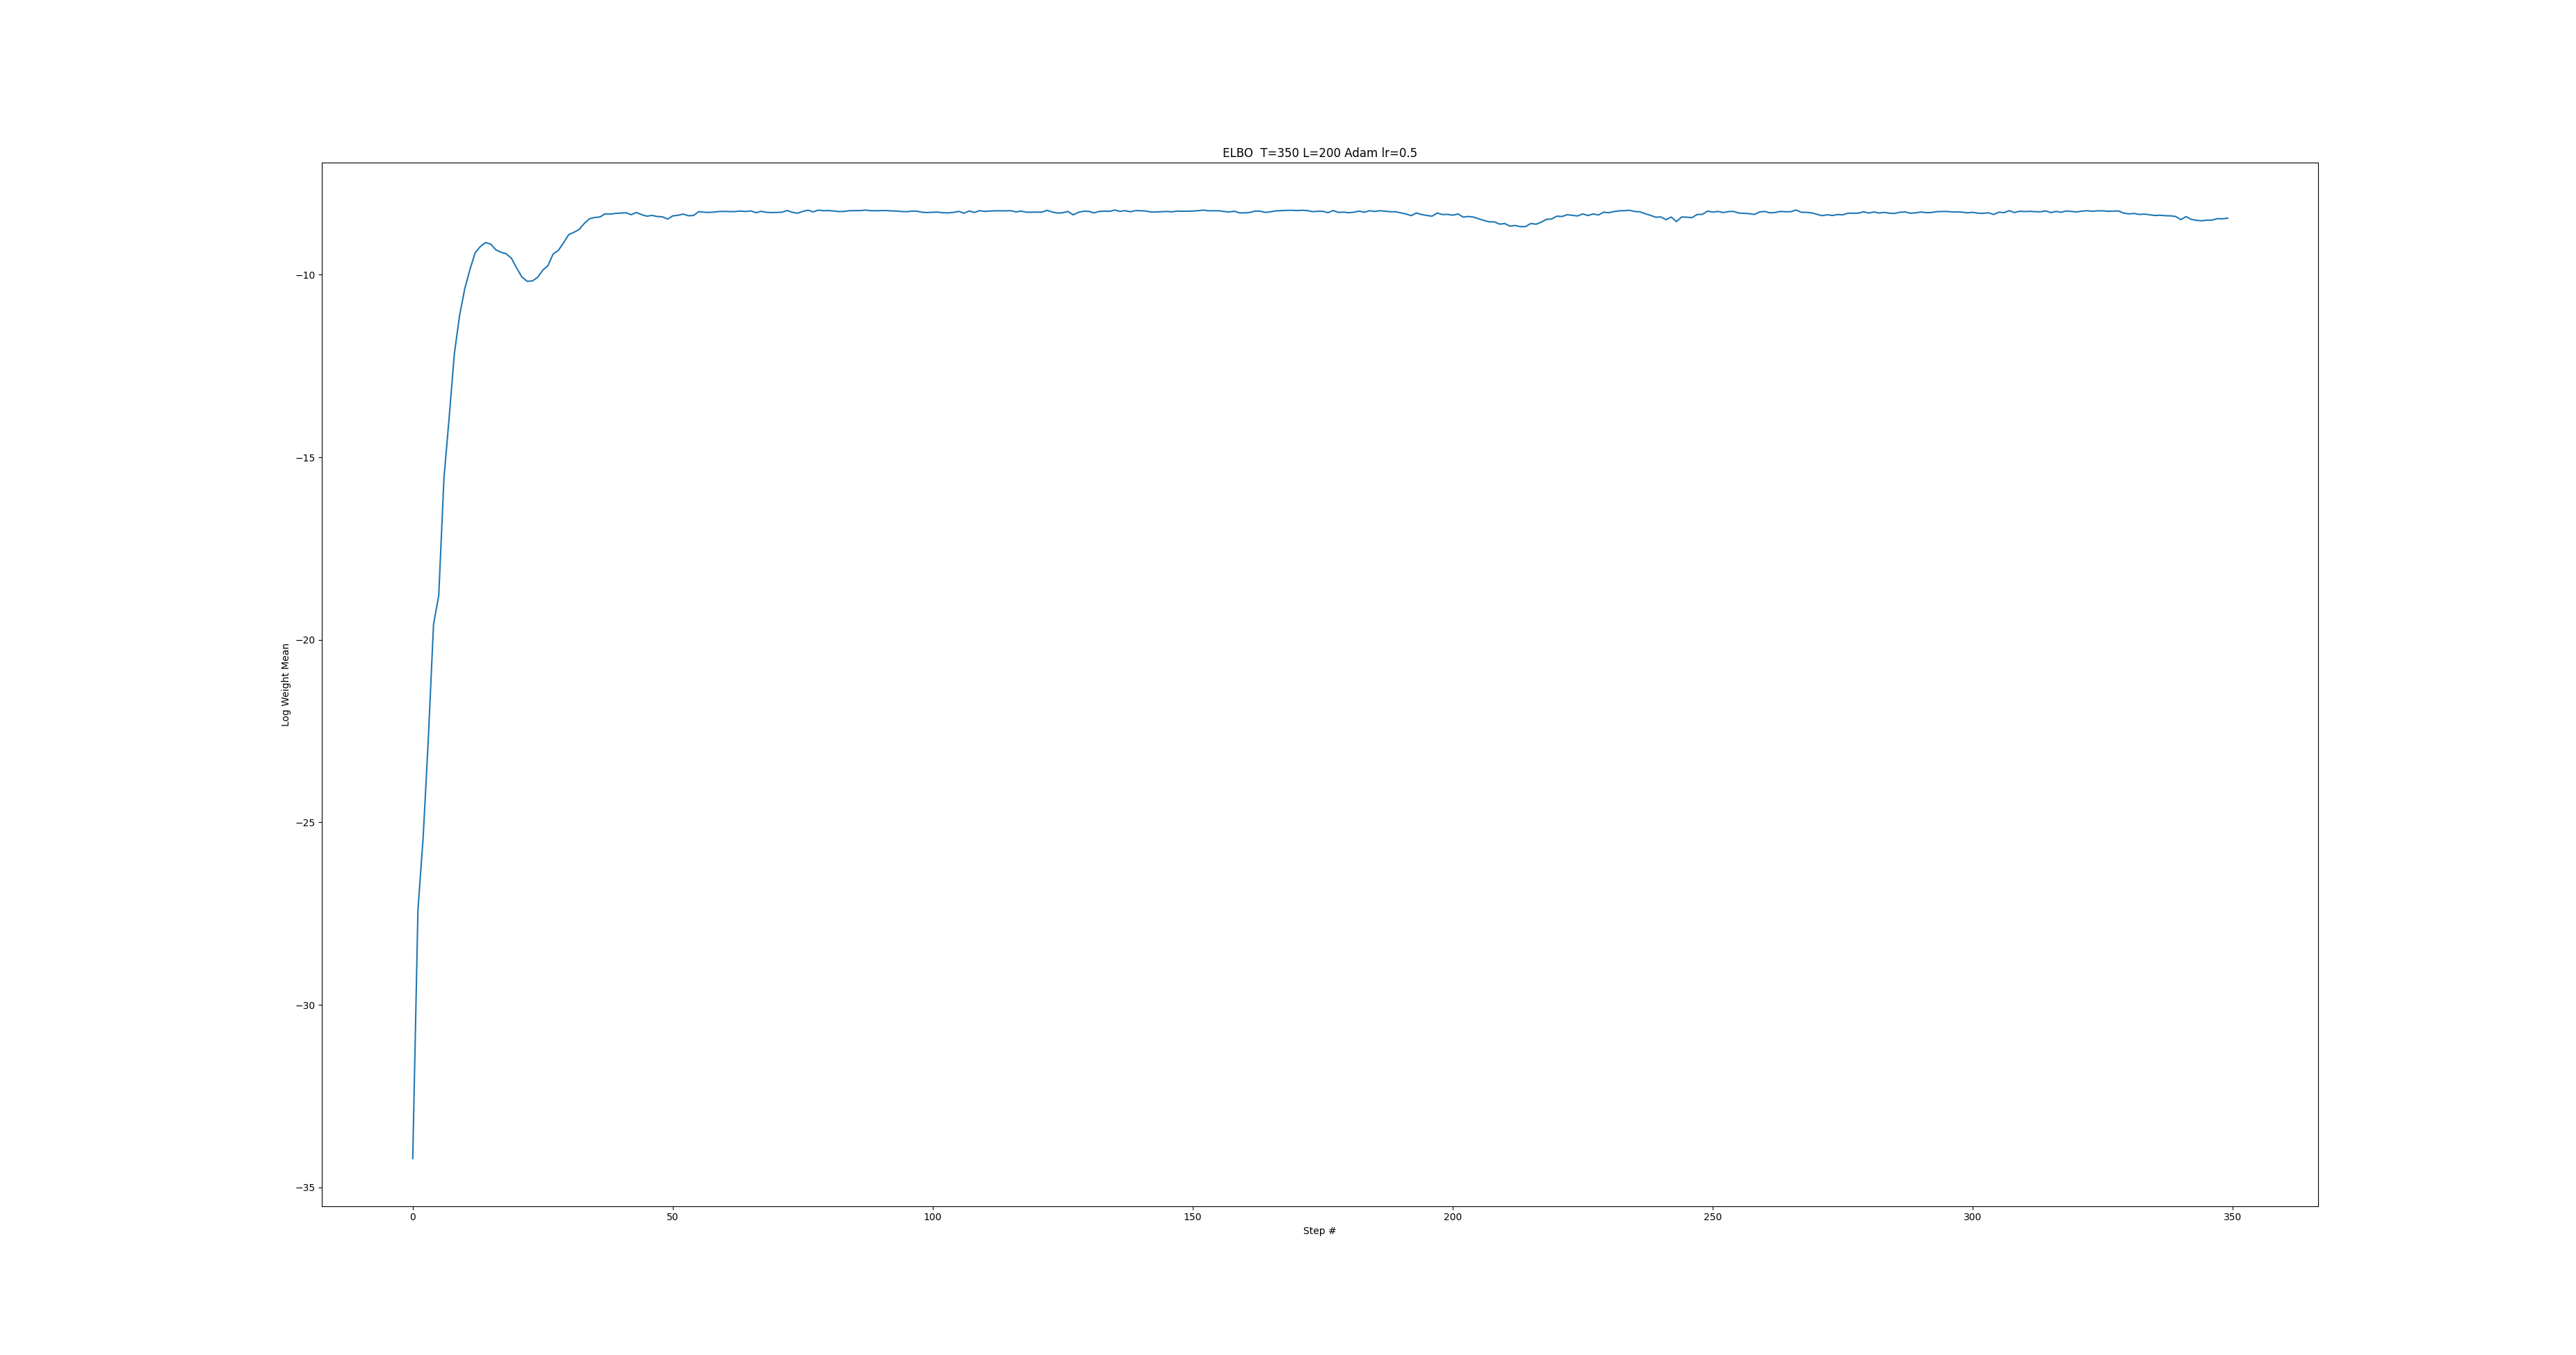
\includegraphics[width=\linewidth]{Figures/elbo_1Adam7.png}
	\captionof{figure}{ELBO plot}
\end{center}
\begin{center}
	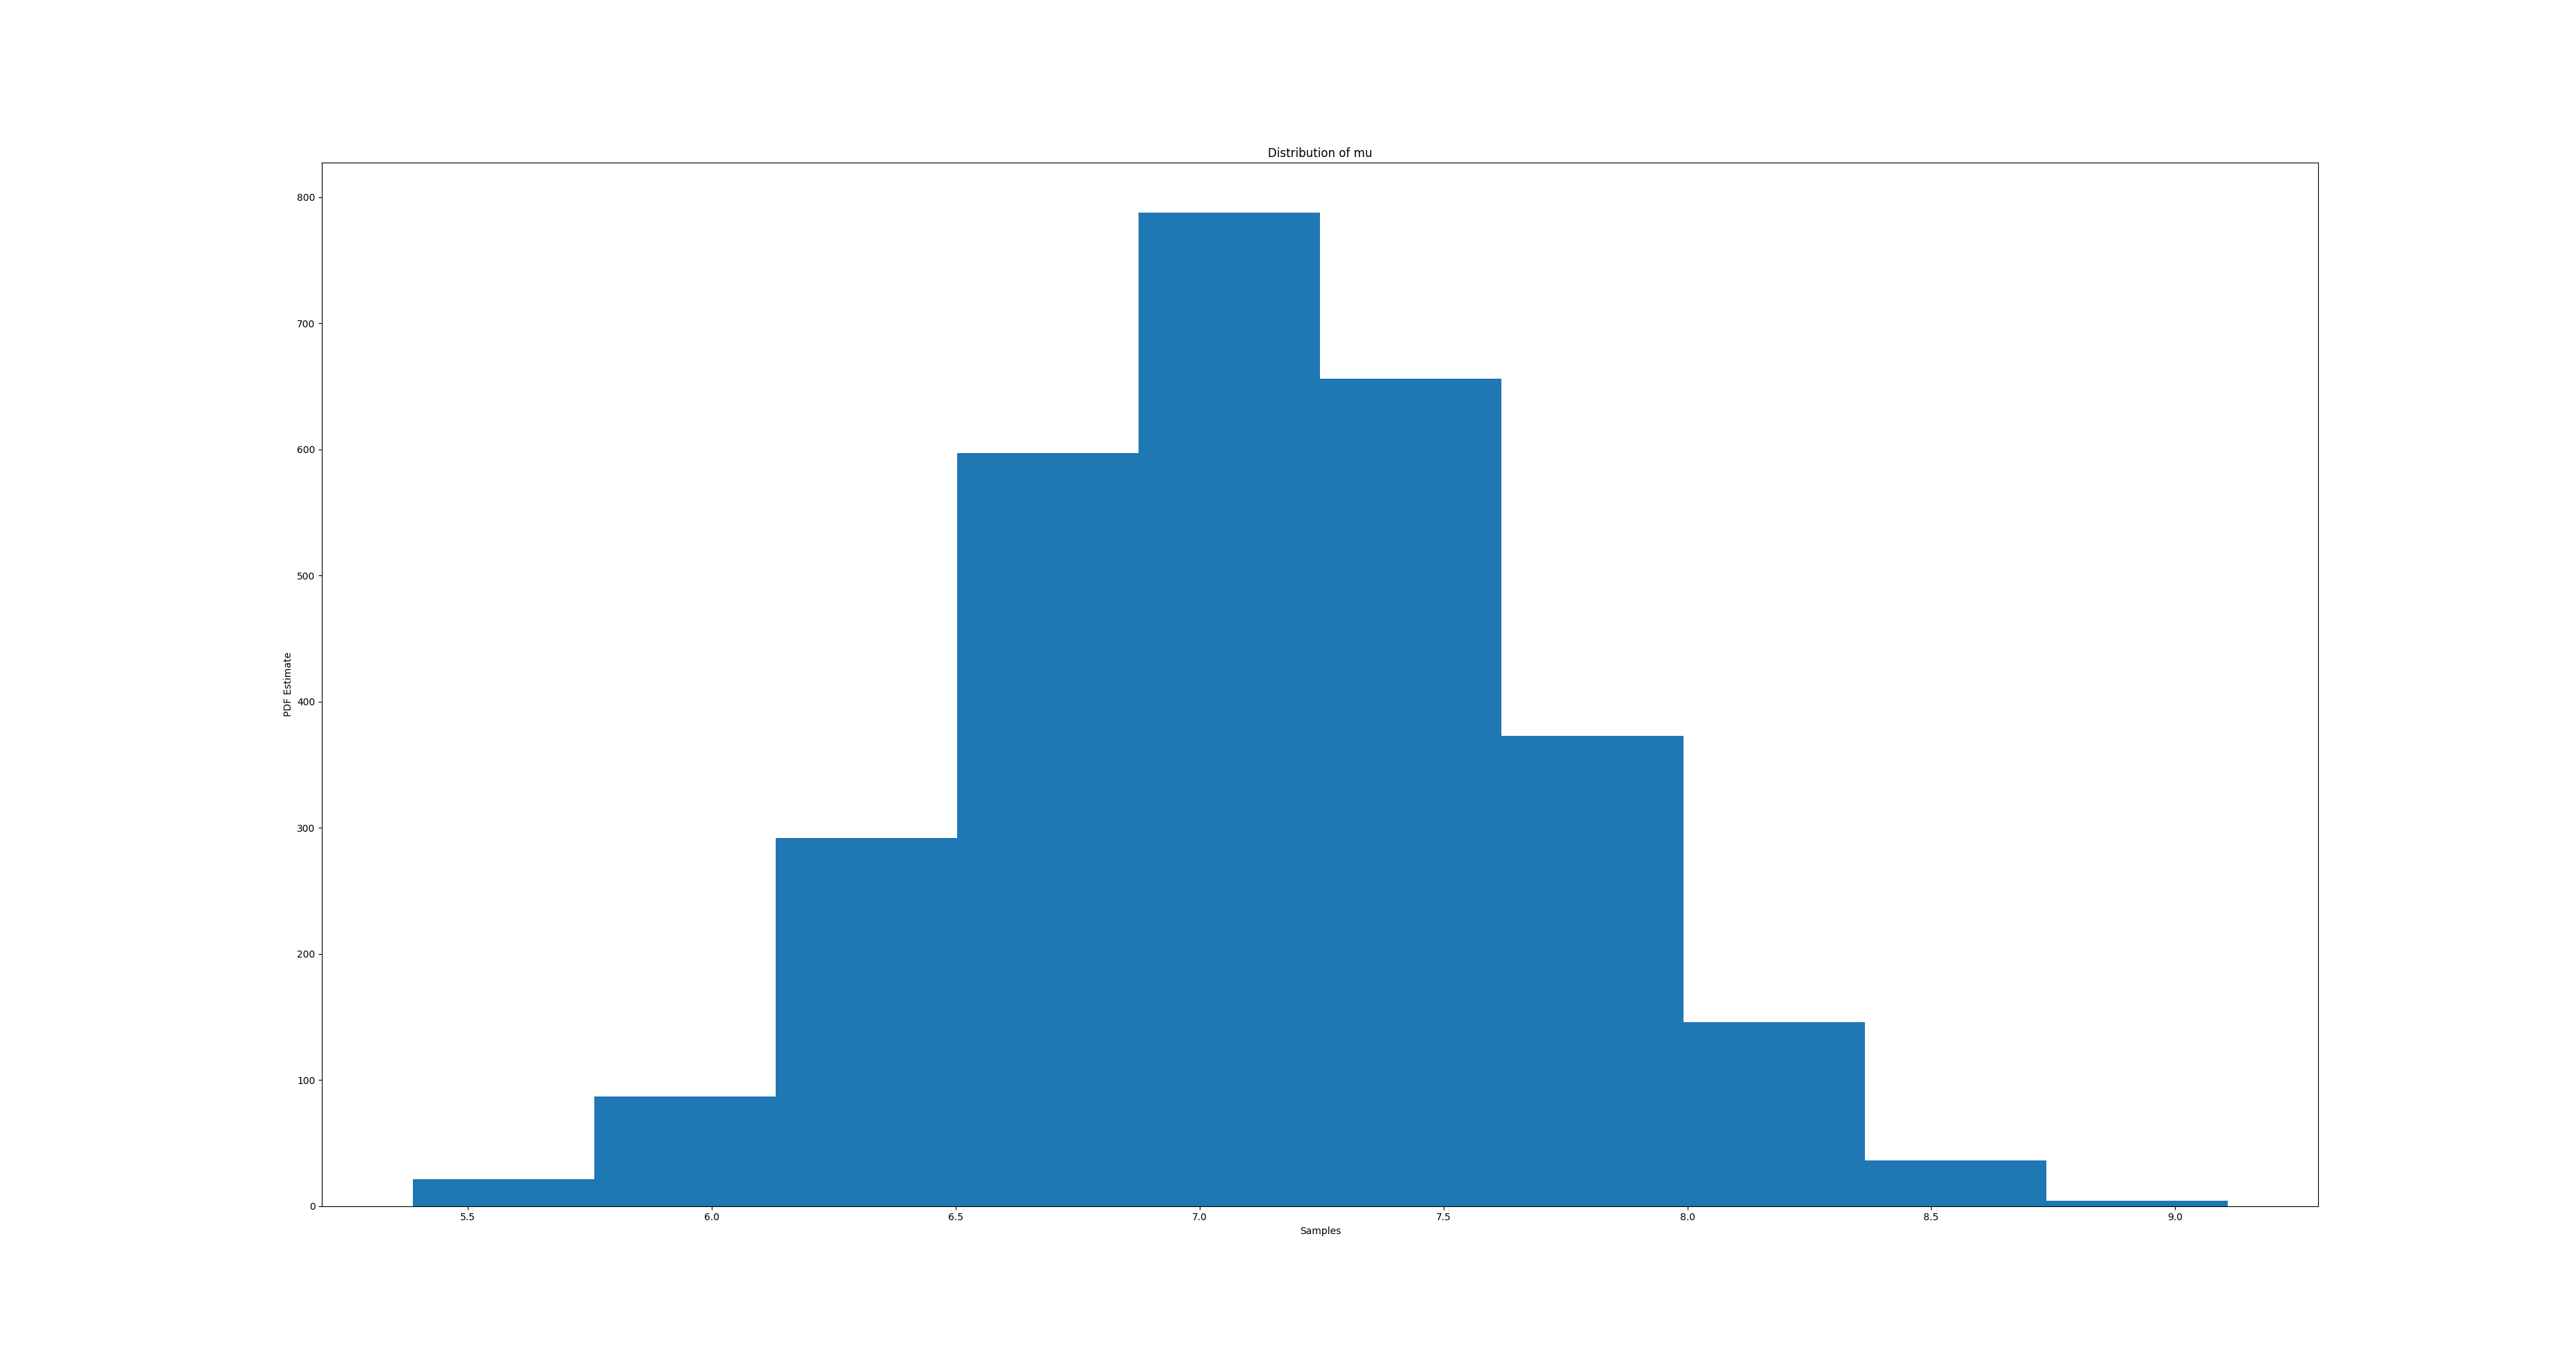
\includegraphics[width=\linewidth]{Figures/distMu_1_3.png}
	\captionof{figure}{Estimate of Distribution $\mu$ from $\mathcal{Q}$}
\end{center}
\begin{center}
	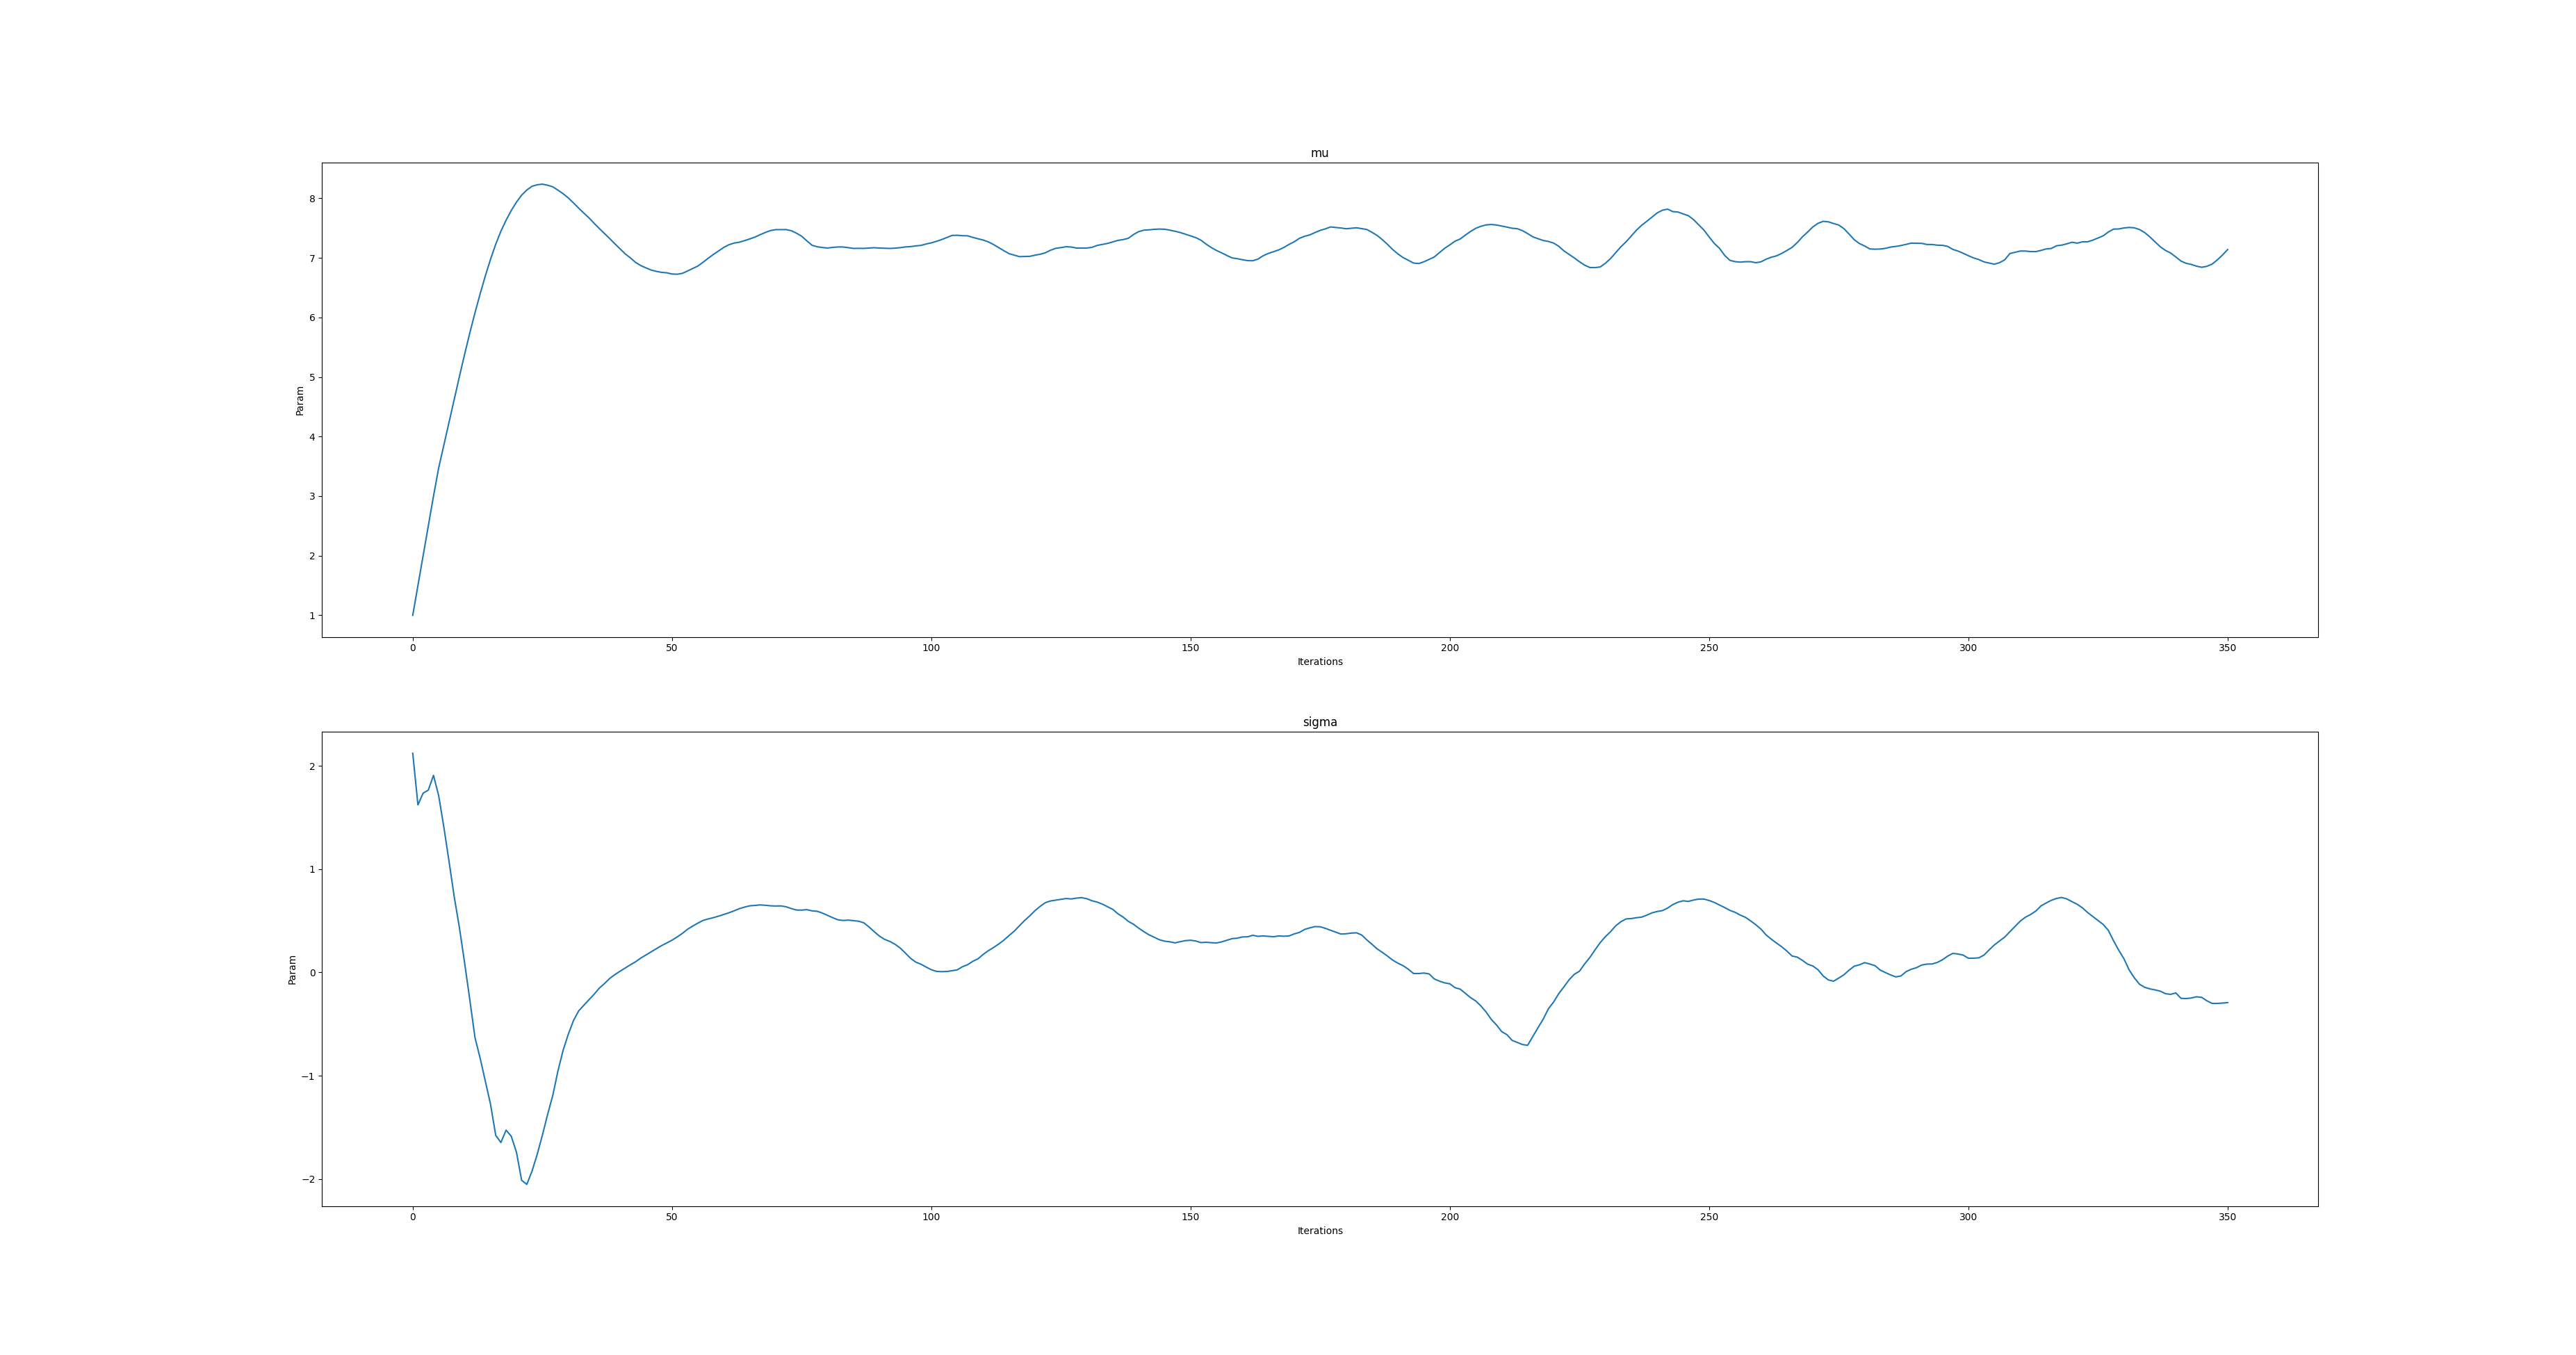
\includegraphics[width=\linewidth]{Figures/muSigma_1_3.png}
	\captionof{figure}{Parameters for $\mathcal{Q}$ for $\mu$ and $\Sigma$ over iterations}
\end{center}
\subsection{Program 2}
Number of samples per optimization is: 200, number of optimization steps is: 350, Adam learning rate: 0.25
\begin{verbatim}
Collect samples denoted by program 2:
Elapsed time for program  2 .daphne is:  0:03:02.441880  seconds
Mean of set of samples:  tensor([1.8603, 0.6375])
and variance of samples:  tensor([0.0843, 1.3375])
\end{verbatim}
\begin{center}
	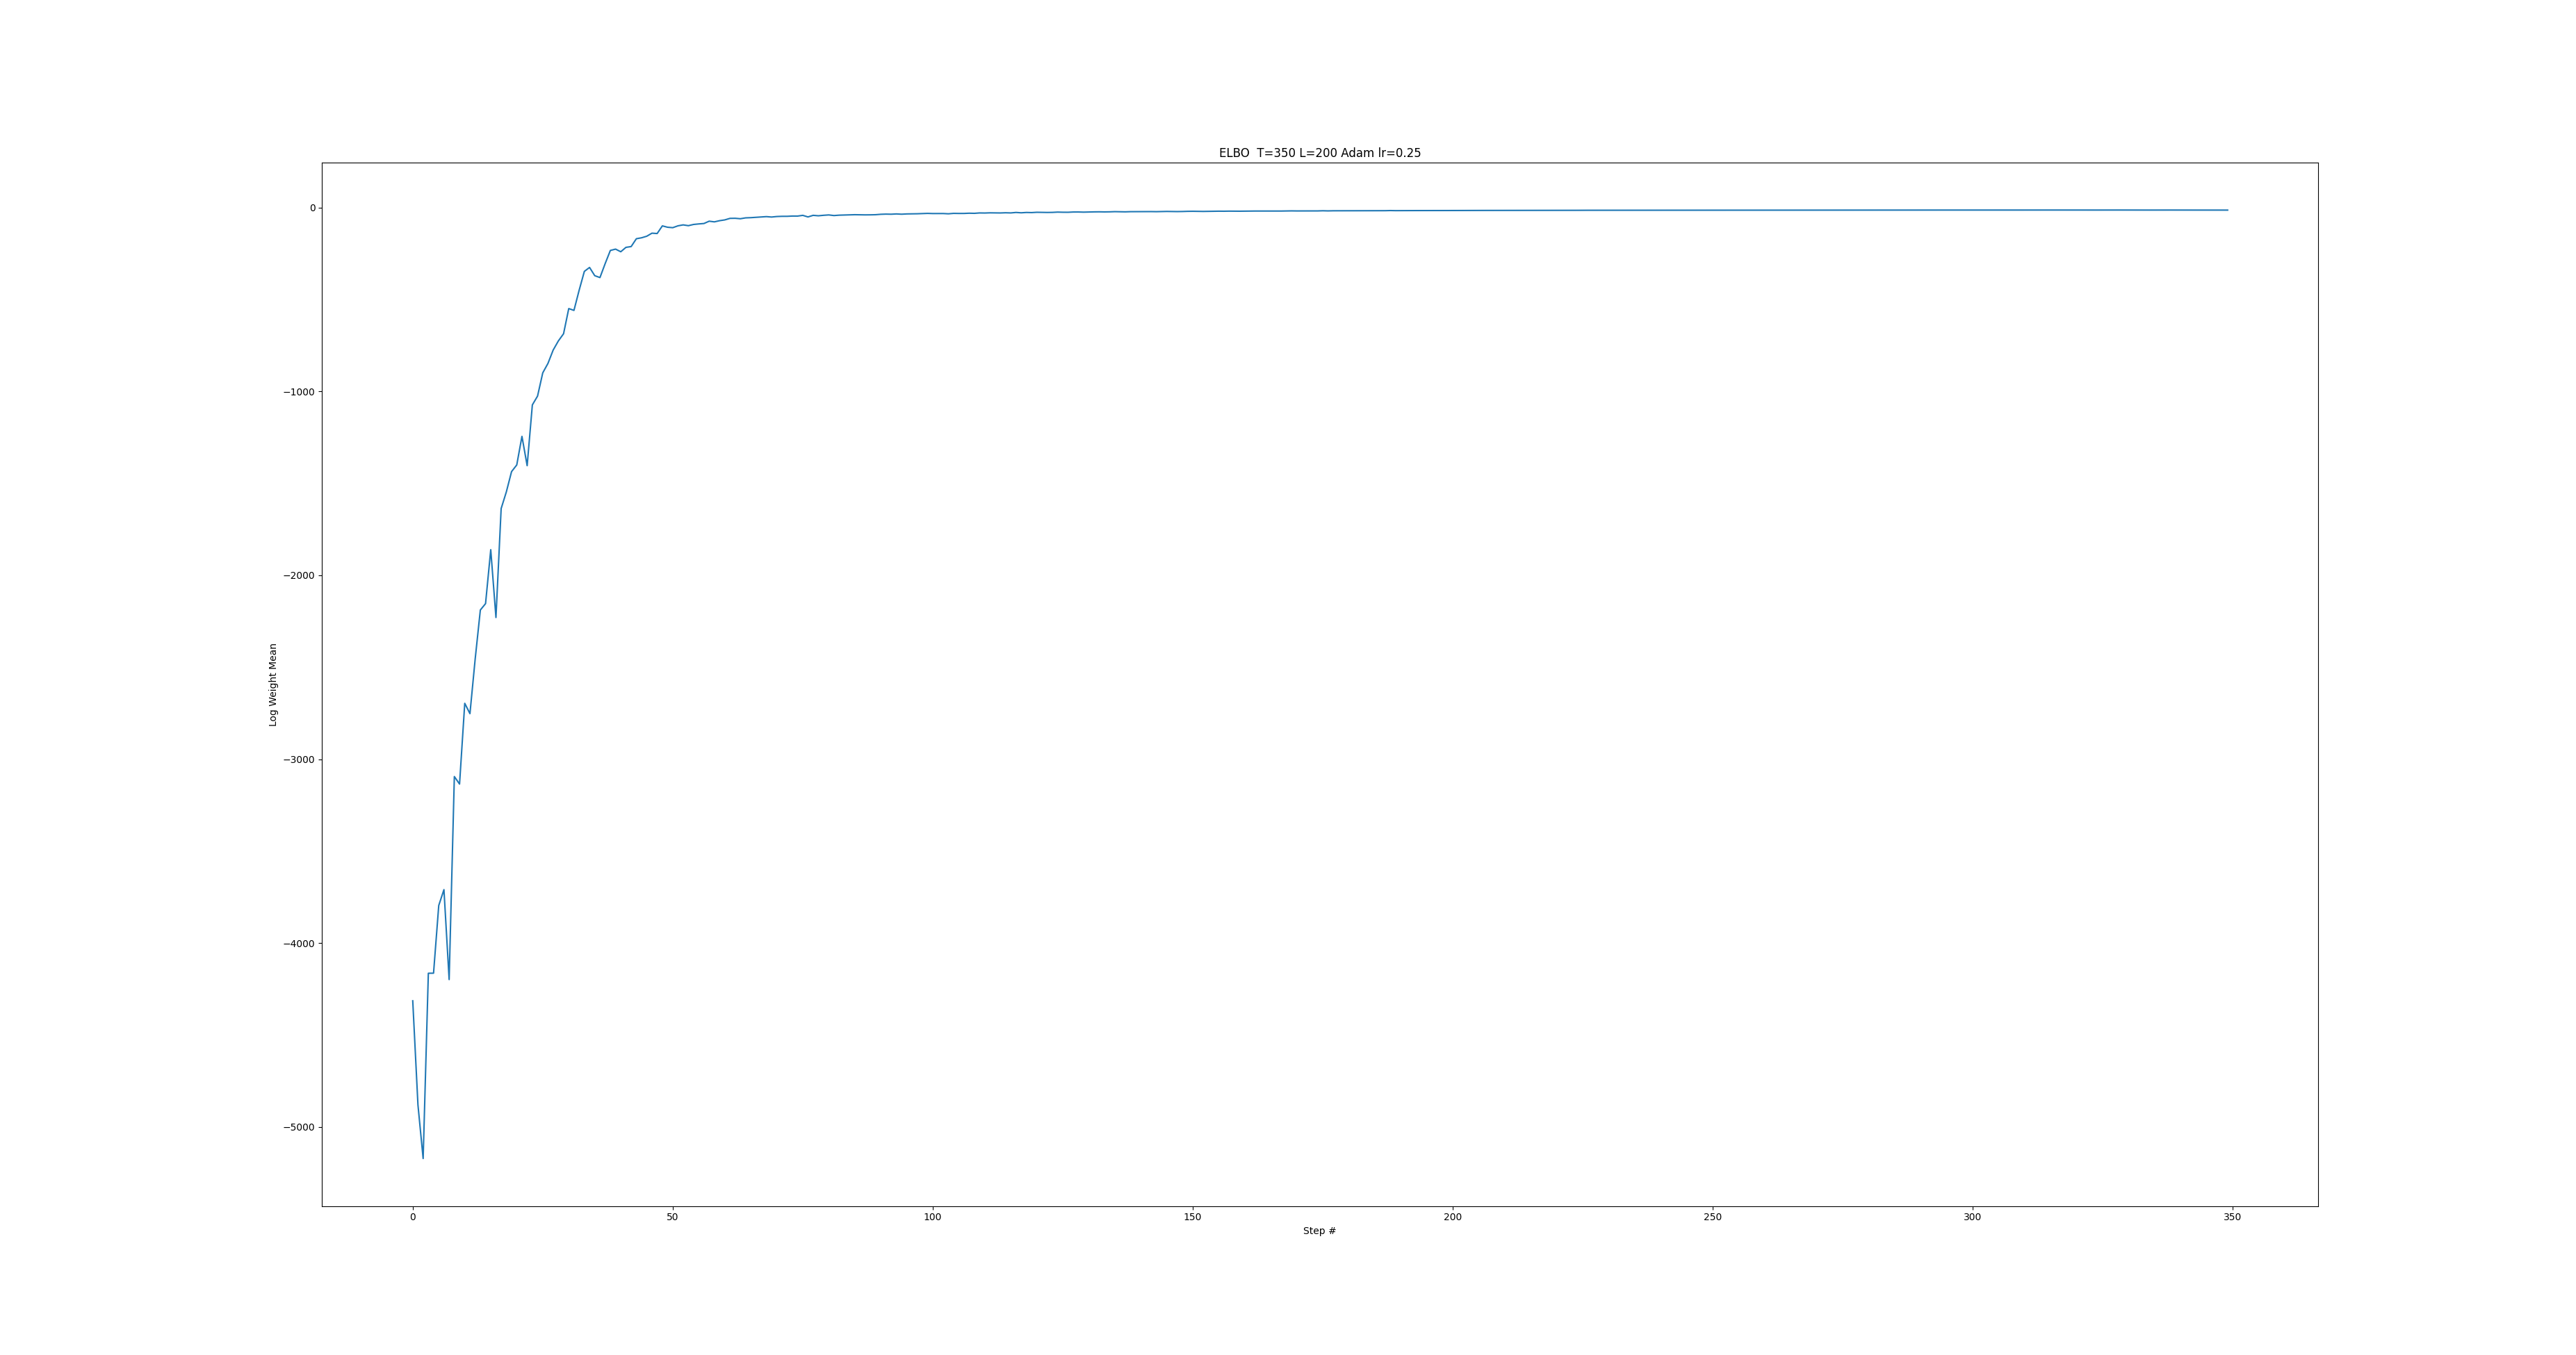
\includegraphics[width=\linewidth]{Figures/elbo_2Adam3.png}
	\captionof{figure}{ELBO plot}
\end{center}
\begin{center}
	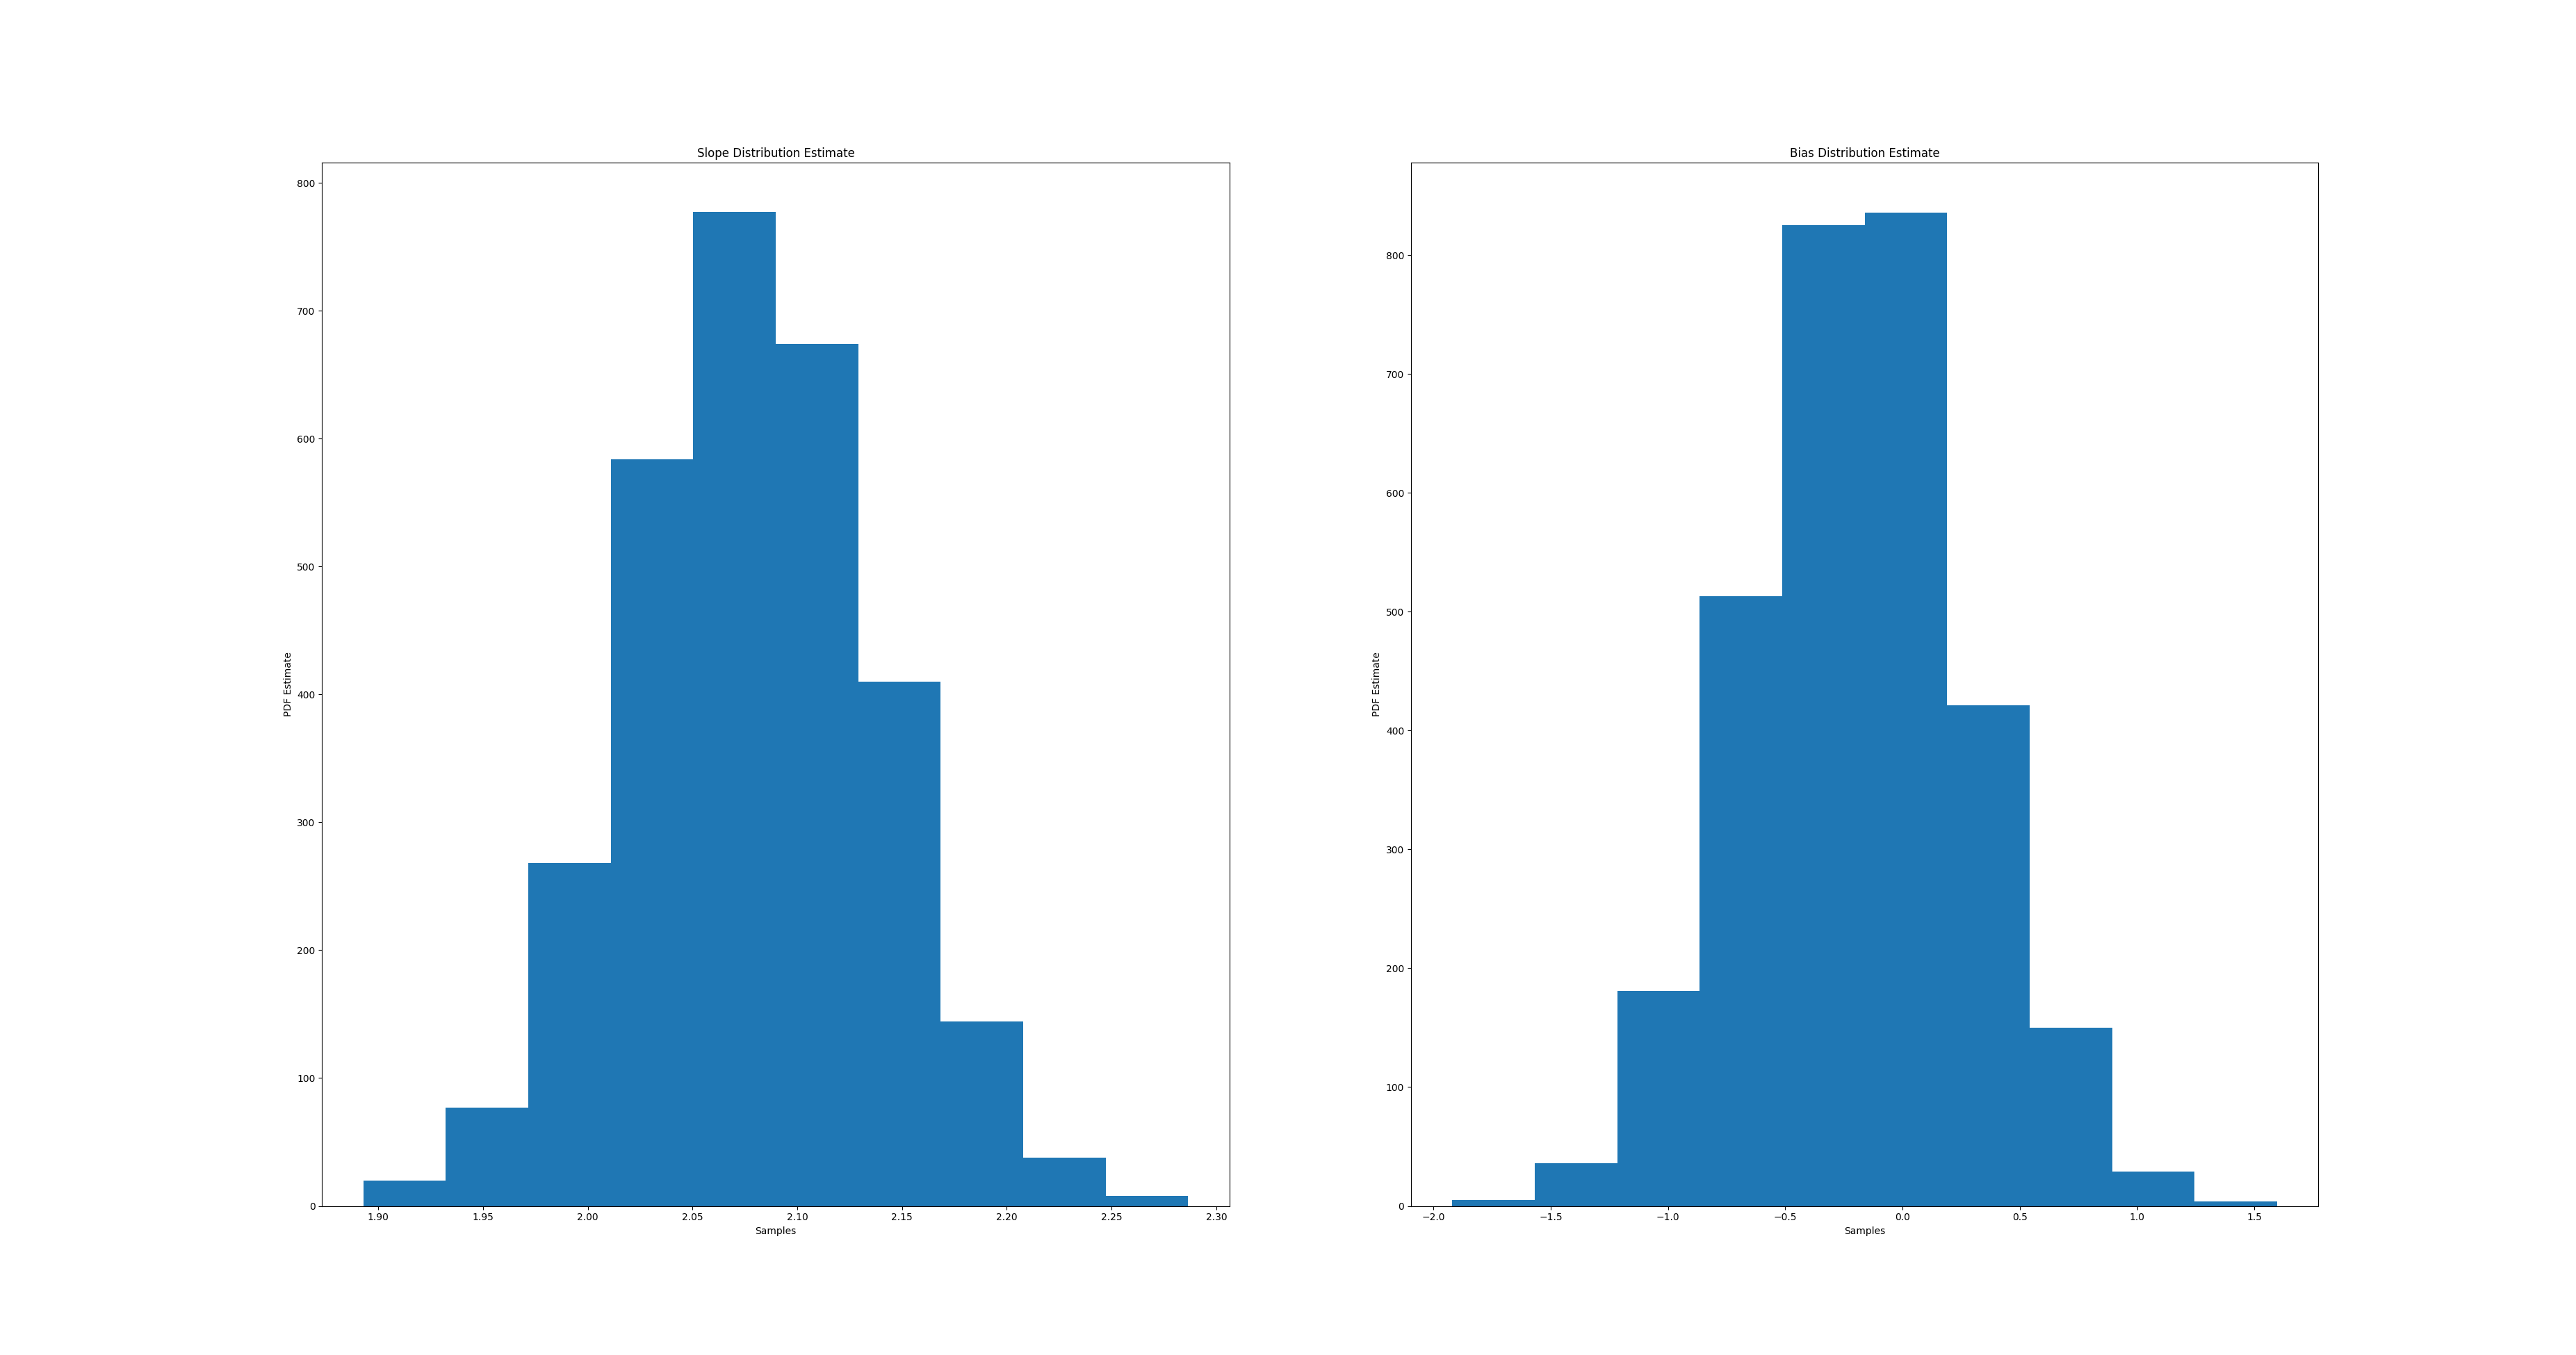
\includegraphics[width=\linewidth]{Figures/distSlopeBias2.png}
	\captionof{figure}{Estimate of Distributions for Slope and Bias from $\mathcal{Q}$ respectively}
\end{center}
\begin{center}
	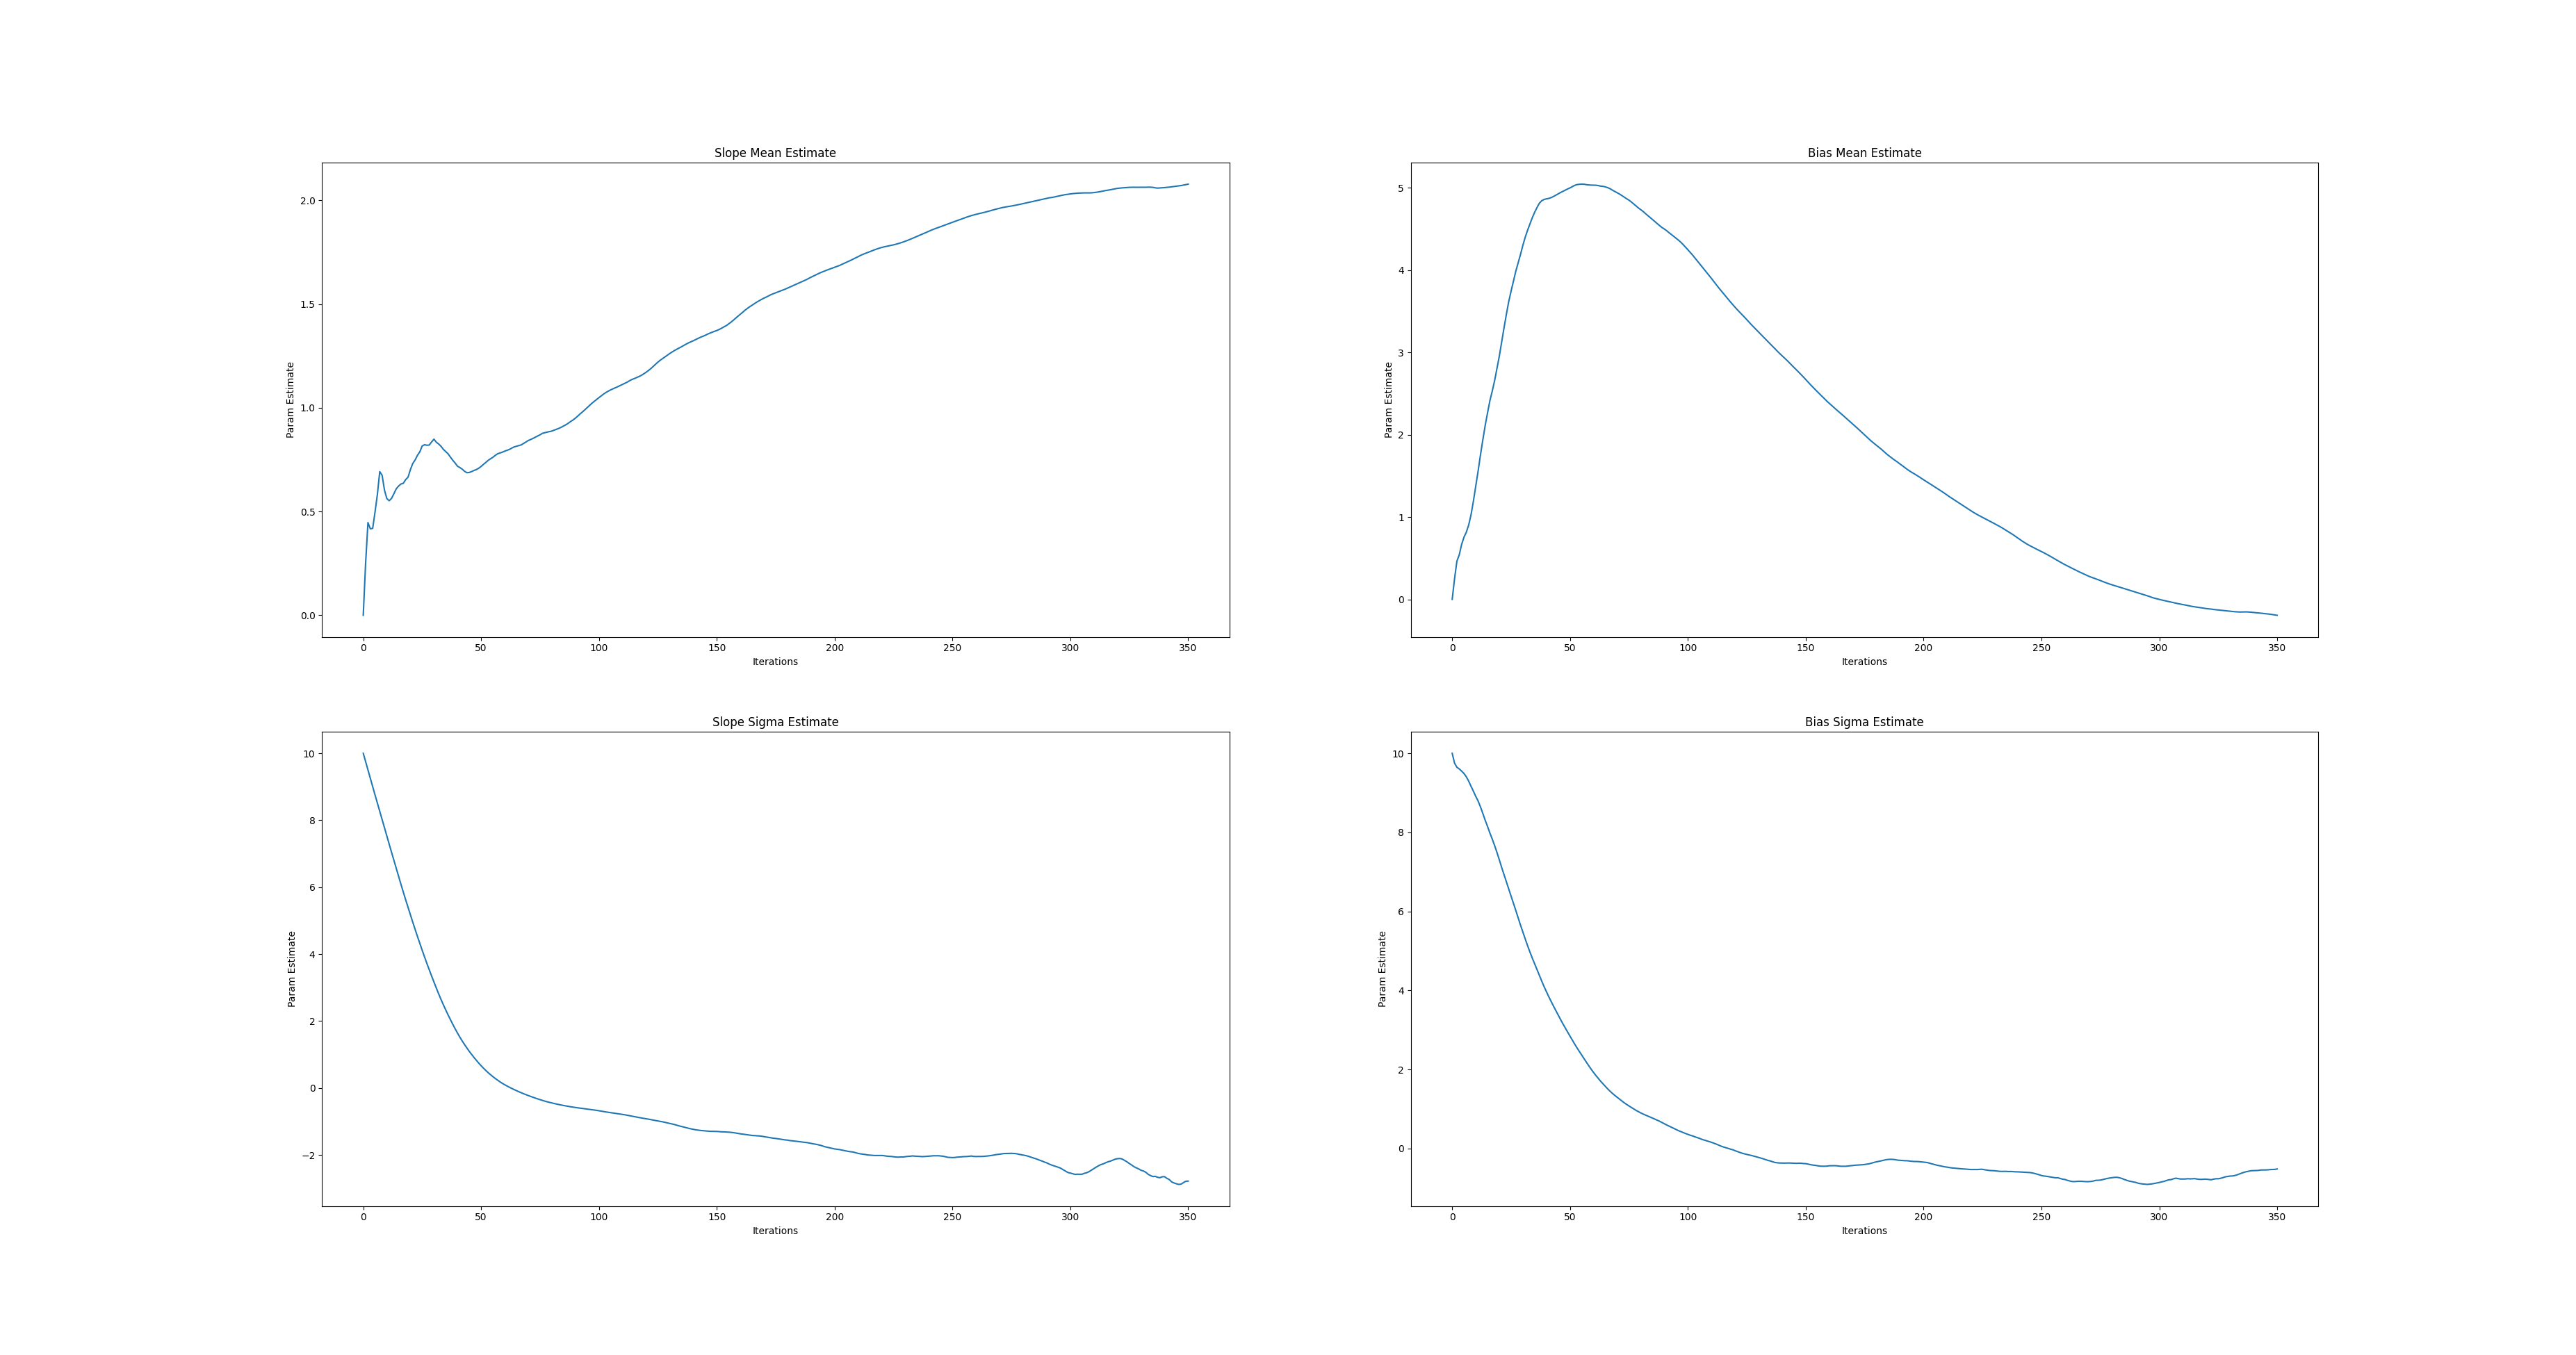
\includegraphics[width=\linewidth]{Figures/muSigP2_2.png}
	\captionof{figure}{Parameters for $\mathcal{Q}$ for Slope and Bias over iterations}
\end{center}
\subsection{Program 3}
Number of samples per optimization is: 25, number of optimization steps is: 350, Adam learning rate: 0.05
\begin{verbatim}
Collect samples denoted by program 3:
Elapsed time for program  3 .daphne is:  0:01:49.841174  seconds
Mean of samples:  tensor(0.5729)
and variance of samples:  tensor(0.2132)
\end{verbatim}
\begin{center}
	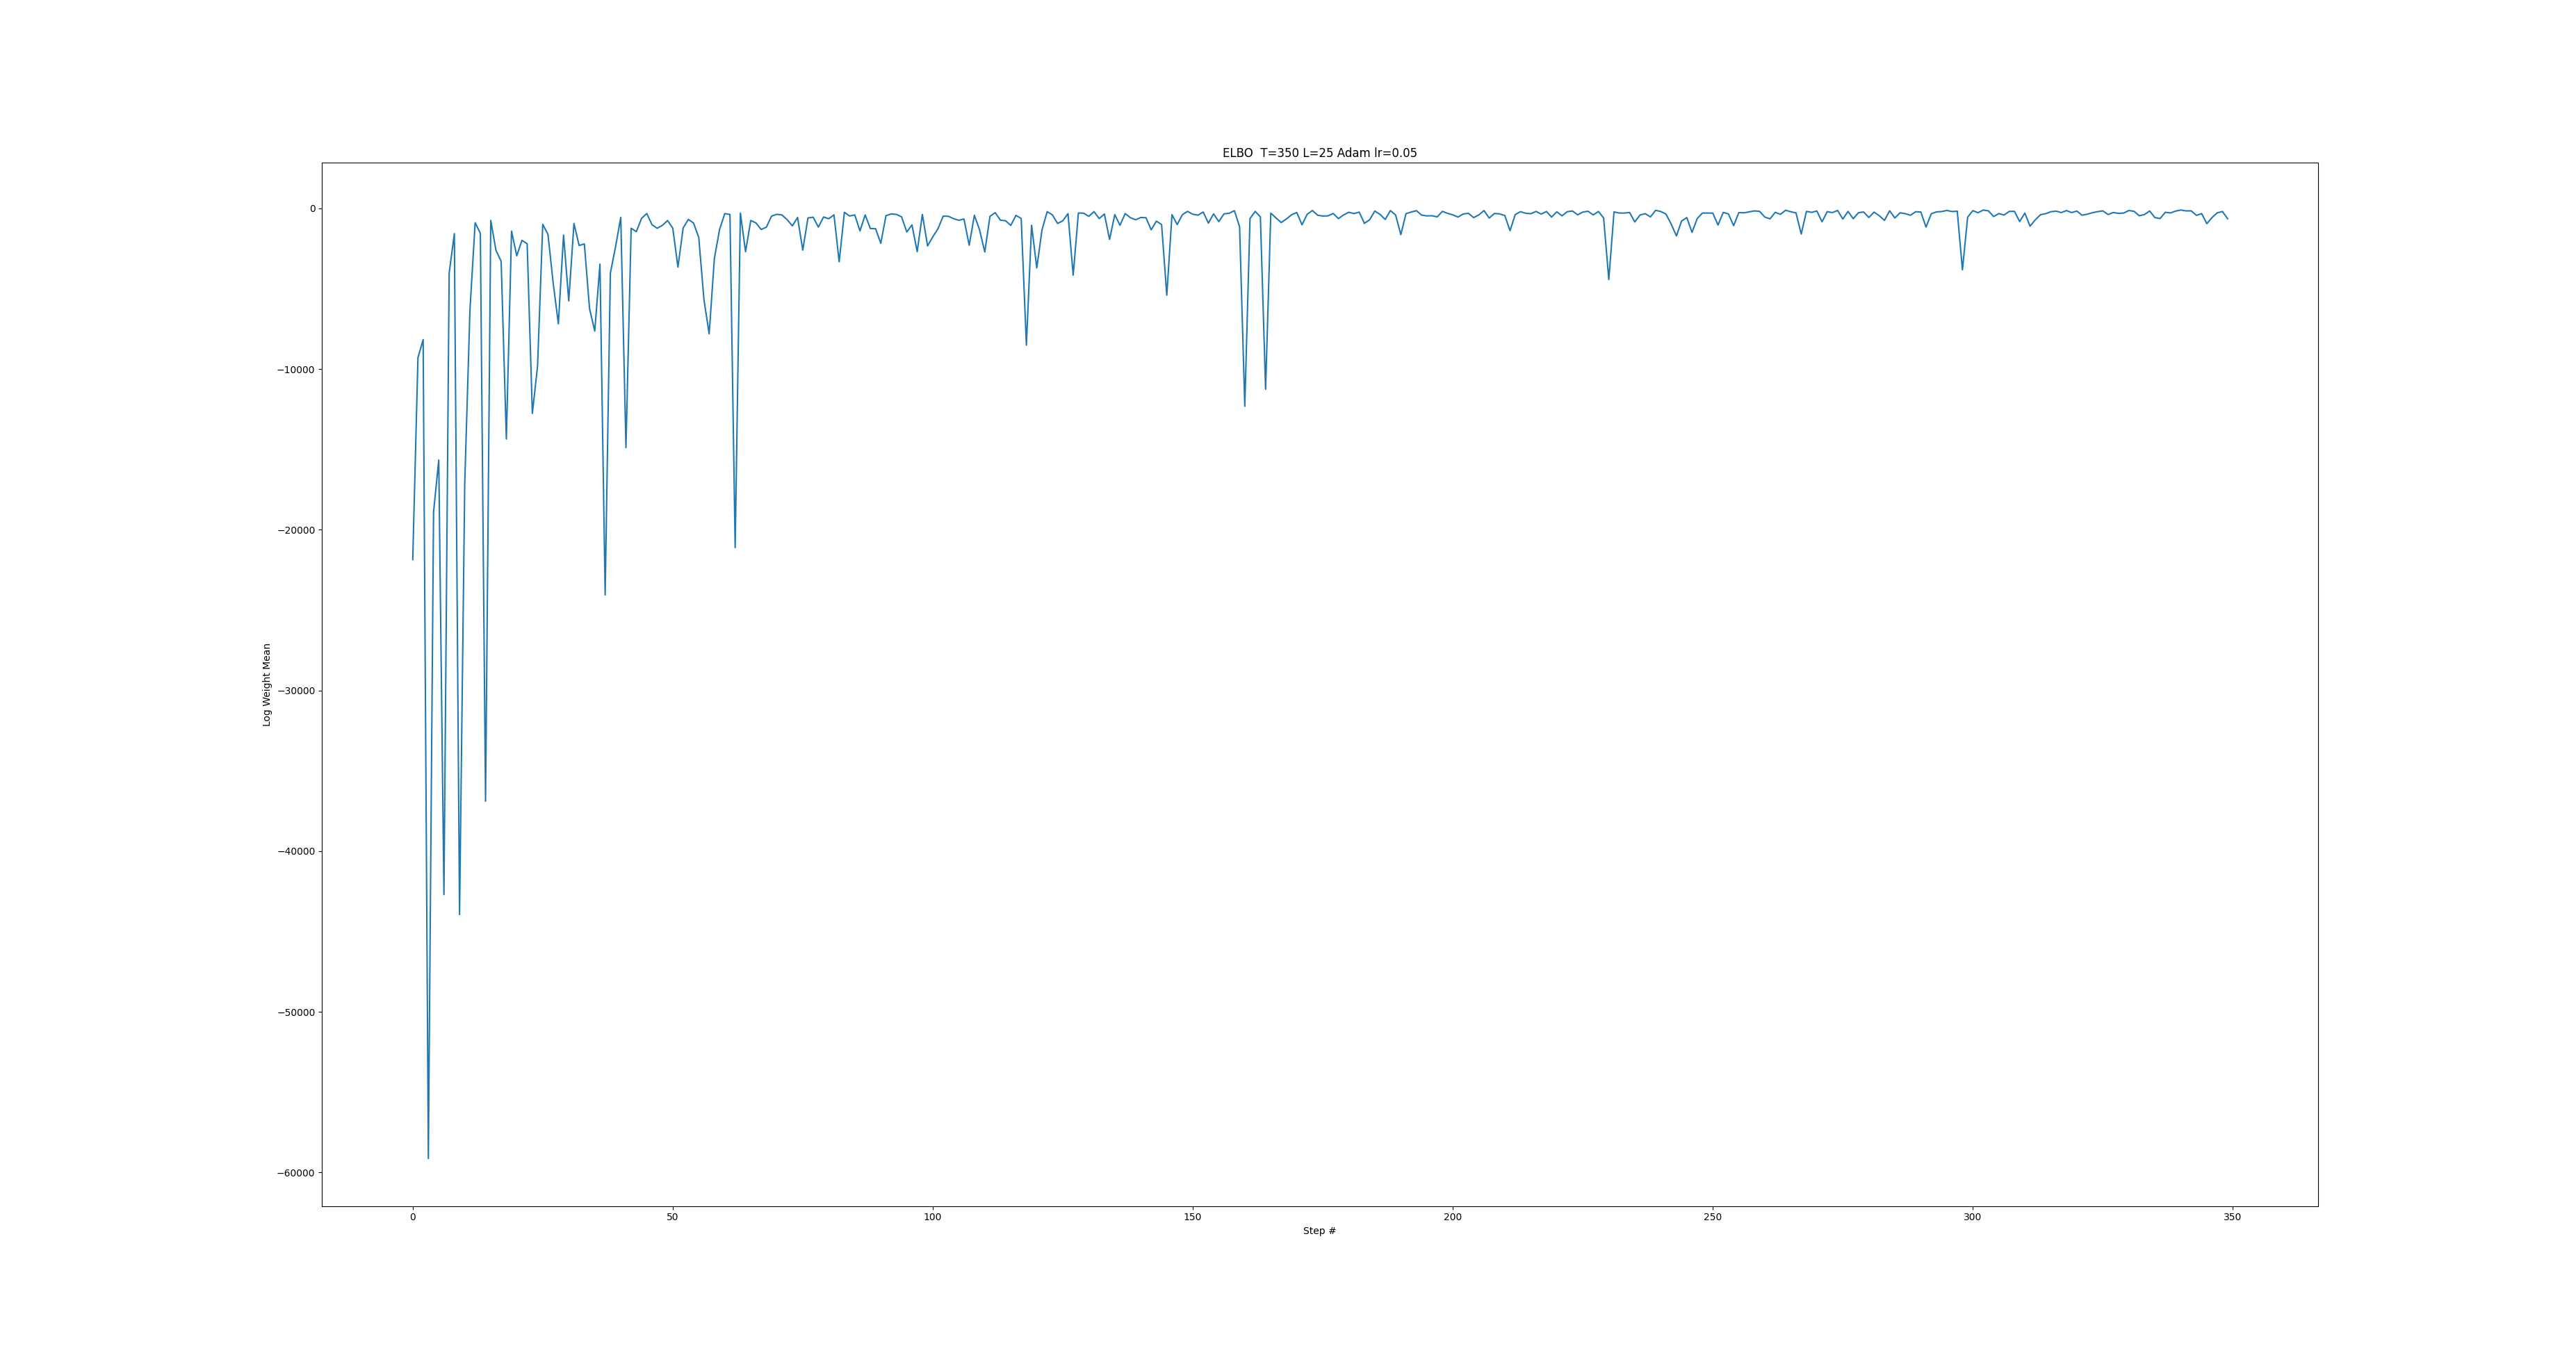
\includegraphics[width=\linewidth]{Figures/elbo_3Adam3.png}
	\captionof{figure}{ELBO plot}
\end{center}
\begin{center}
	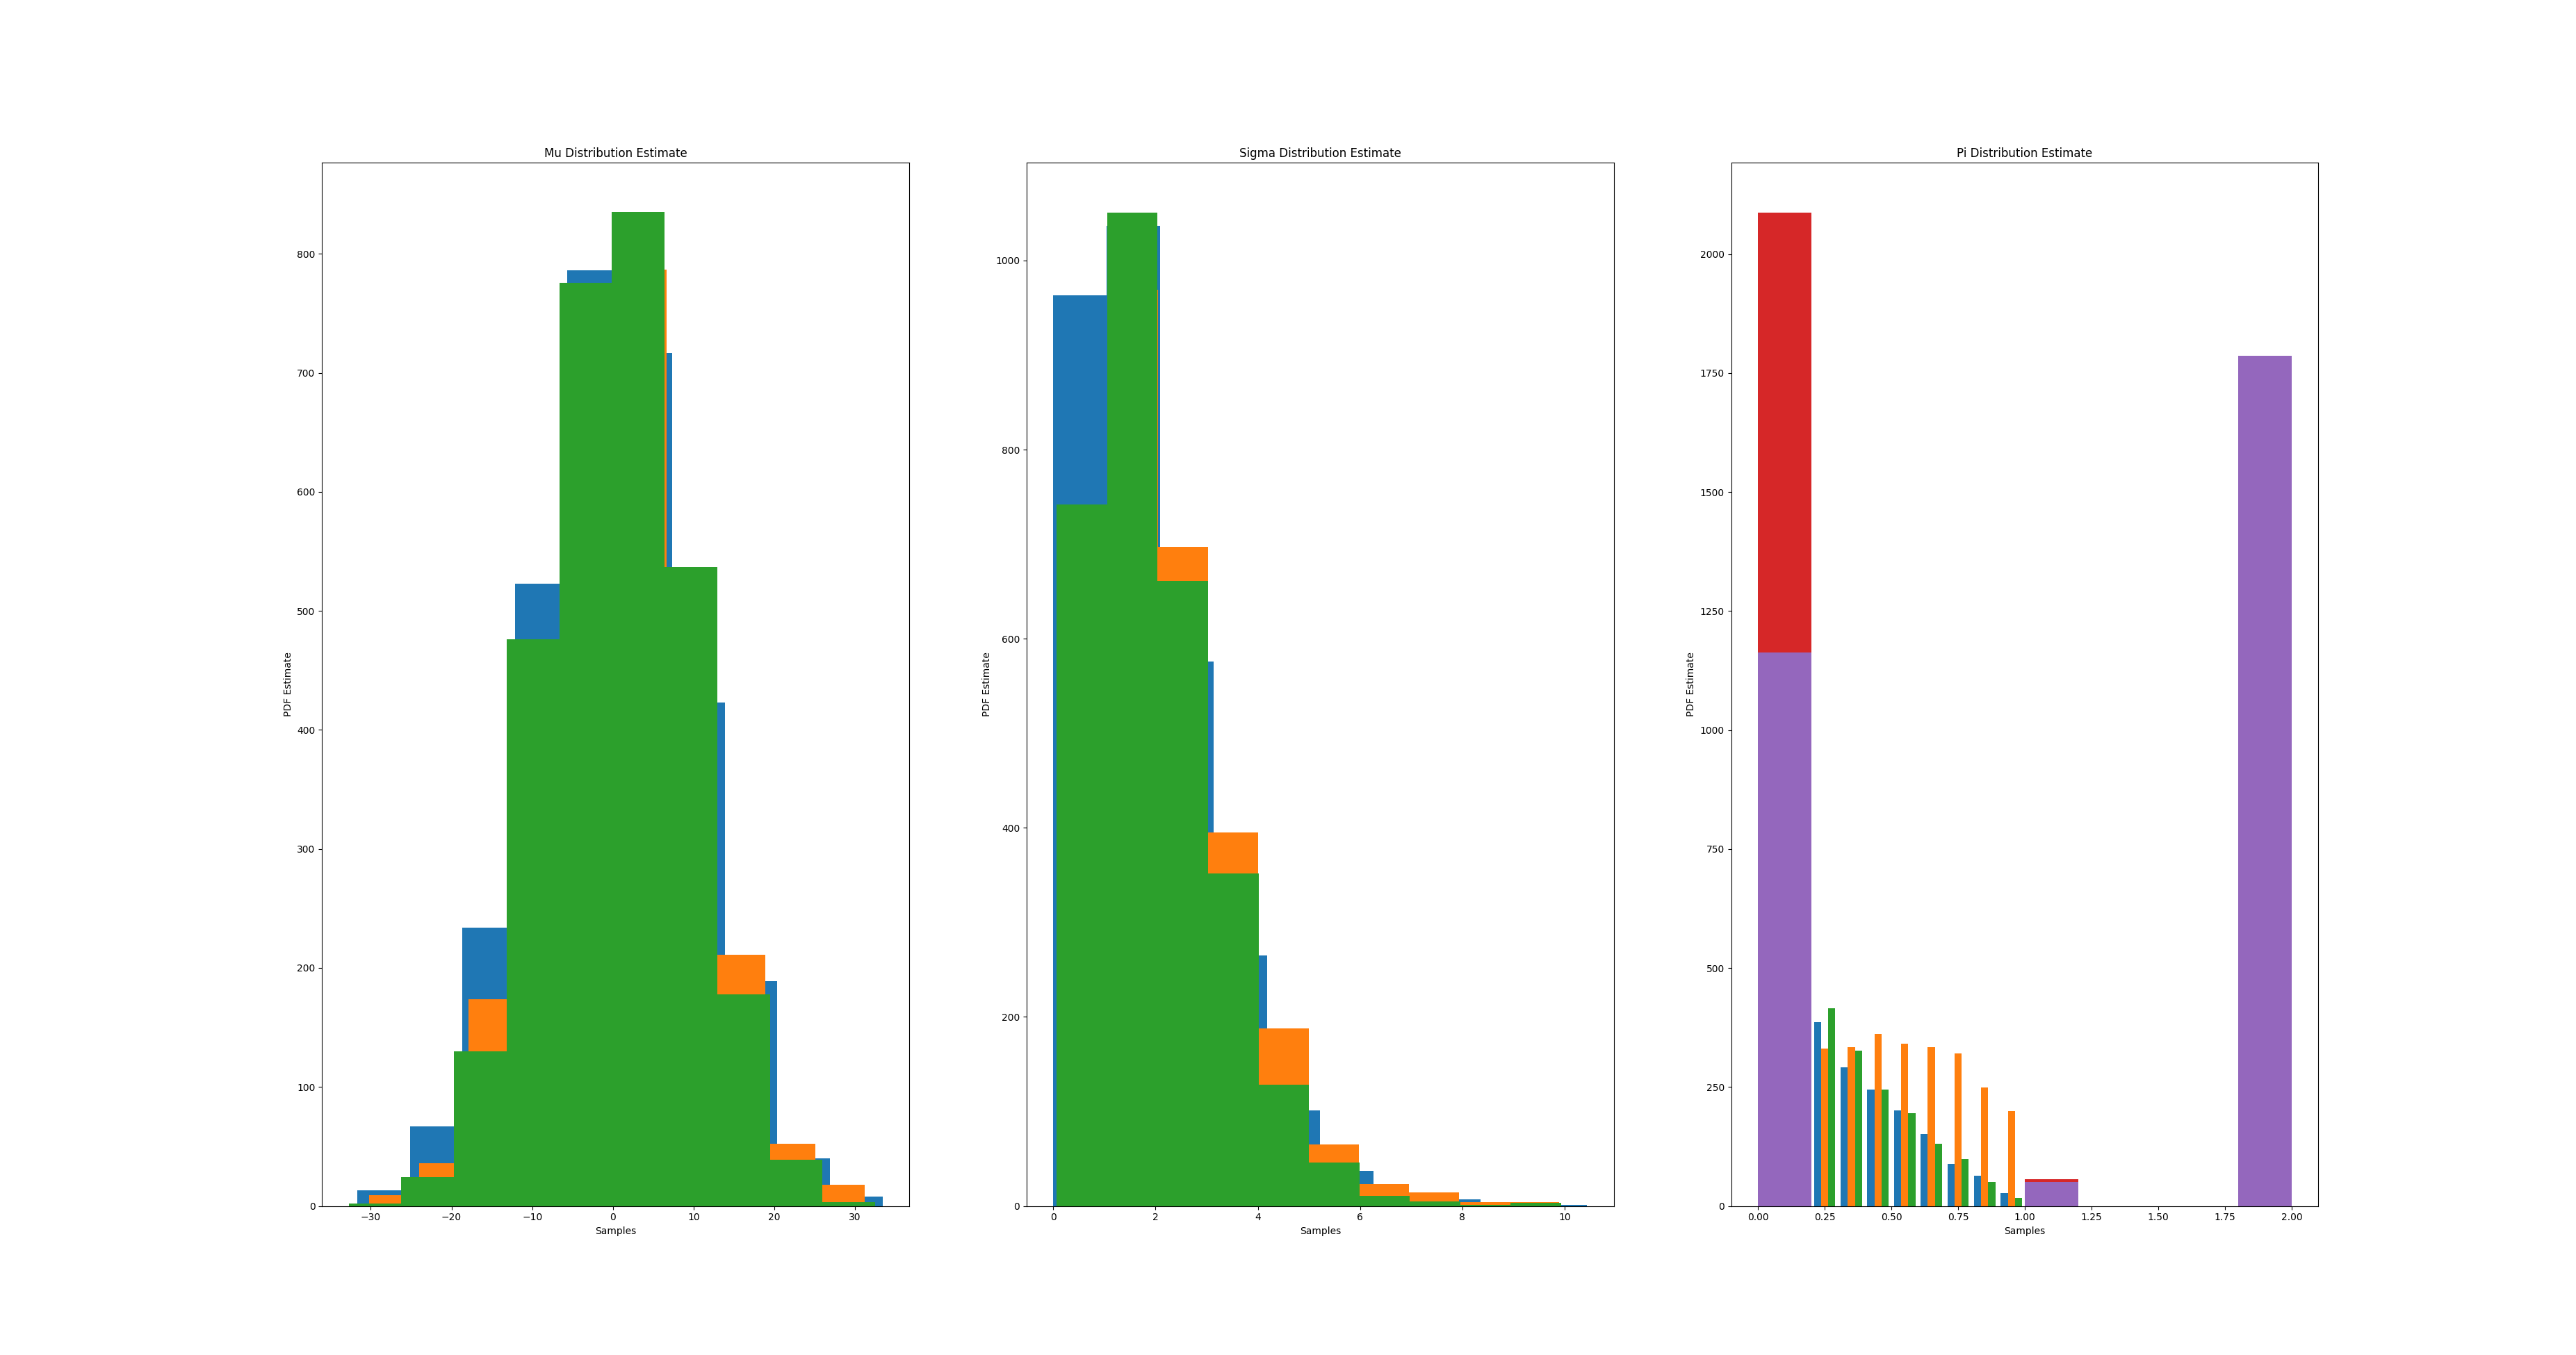
\includegraphics[width=\linewidth]{Figures/distEst3.png}
	\captionof{figure}{Estimates of Distributions for the 3 Modes ($\mu$ and $\Sigma$) and $\Pi$}
\end{center}
During optimization there are sudden jumps where the ELBO drops significantly likely arising from the fact that the modes switch, i.e. sampling from one mode for awhile and then sampling from another. In these instances a sudden drop in the importance weights will arise from estimating the distribution from the "wrong" place. The convergence back to the previous ELBO is quick, however this bouncing around makes optimization hard.

Optimizing with a mix of discrete and continuous random variables is a difficult problem to optimize. Here the Dirichelet distribution would make pathwise gradient optimization impossible because of the discontinuity when switching from one mode to the other.
\subsection{Program 4}
Number of samples per optimization is: 150, number of optimization steps is: 200, Adam learning rate: 0.1
\begin{verbatim}
Collect samples denoted by program 4:
Elapsed time for program  4 .daphne is:  0:32:30.898768  seconds
Mean of samples  W0 :  tensor([[-0.0538],
[ 0.0759],
[-0.0523],
[-0.4615],
[-0.0378],
[-0.0117],
[-0.0077],
[-0.0430],
[ 0.2541],
[-0.2181]])
and variance of samples  W0 :  tensor([[0.5128],
[0.5521],
[0.2950],
[0.4300],
[0.4077],
[0.2621],
[0.6241],
[0.5681],
[0.4060],
[0.3981]])
Mean of samples  b0 :  tensor([[ 0.0283],
[-0.1436],
[ 0.0596],
[-0.1415],
[-0.0643],
[-0.1060],
[ 0.0333],
[-0.3151],
[ 0.2745],
[ 0.2415]])
and variance of samples  b0 :  tensor([[0.3771],
[0.3458],
[0.4271],
[0.3895],
[0.4588],
[0.3073],
[0.4415],
[0.2625],
[0.4780],
[0.2059]])
Mean of samples  W1 :  tensor([[-0.3377,  0.1622,  0.2904,  0.3412, -0.0154, -0.2529,  0.1761,  0.6720,
-0.1905,  0.1341],
[ 0.6109, -0.0588,  0.1595, -0.2266, -0.2677, -0.1859,  0.2364,  0.0217,
-0.0459,  0.0779],
[-0.0839, -0.2009, -0.3588, -0.1991,  0.1542, -0.0972,  0.2010, -0.1792,
-0.1038, -0.0384],
[ 0.0038,  0.0847, -0.0733, -0.2610,  0.0972,  0.1078, -0.0553,  0.2599,
-0.1014, -0.2961],
[ 0.0242,  0.0829, -0.0083,  0.2522,  0.1779,  0.1928, -0.2569, -0.4040,
-0.1642,  0.0741],
[ 0.1149, -0.2028, -0.1752, -0.1942, -0.3036,  0.5337,  0.0388,  0.1312,
-0.0115, -0.0357],
[ 0.4245,  0.3058, -0.2490,  0.0654,  0.1084, -0.0598,  0.3495,  0.0311,
-0.2384,  0.5183],
[-0.1928, -0.1891, -0.2955, -0.3391,  0.2615, -0.1450, -0.2682, -0.1339,
-0.2855,  0.1191],
[ 0.2049, -0.0804, -0.1176, -0.0216, -0.0917, -0.0542,  0.1835,  0.0915,
-0.1915, -0.0375],
[-0.0047,  0.1943, -0.1376, -0.2776,  0.0288,  0.1535,  0.0938, -0.0937,
-0.1021, -0.0475]])
and variance of samples  W1 :  tensor([[0.3923, 0.4234, 0.4946, 0.2481, 0.4493, 0.2450, 0.2761, 0.3342, 0.3820,
0.3278],
[0.4420, 0.3859, 0.4415, 0.4125, 0.3175, 0.3814, 0.3217, 0.4444, 0.3659,
0.3045],
[0.3325, 0.4457, 0.4203, 0.6208, 0.4533, 0.2631, 0.4323, 0.5770, 0.3698,
0.5566],
[0.3912, 0.3266, 0.3773, 0.3905, 0.5574, 0.6455, 0.5060, 0.3169, 0.4468,
0.4718],
[0.4554, 0.6540, 0.2060, 0.3671, 0.4822, 0.3046, 0.2851, 0.4852, 0.4505,
0.6185],
[0.5007, 0.4577, 0.4148, 0.3821, 0.4859, 0.3172, 0.4985, 0.4503, 0.2416,
0.5182],
[0.4381, 0.5384, 0.4589, 0.3488, 0.5986, 0.4541, 0.4134, 0.3126, 0.2671,
0.3327],
[0.5090, 0.4212, 0.4048, 0.5165, 0.2403, 0.1082, 0.6374, 0.3966, 0.2565,
0.5461],
[0.3849, 0.4273, 0.3088, 0.5978, 0.3867, 0.5247, 0.4416, 0.3489, 0.5252,
0.4045],
[0.3821, 0.3247, 0.4055, 0.5226, 0.4852, 0.3786, 0.3103, 0.4447, 0.6368,
0.3510]])
Mean of samples  b1 :  tensor([[ 0.0669],
[ 0.2564],
[-0.0540],
[-0.3482],
[ 0.1357],
[-0.1493],
[ 0.3596],
[-0.0459],
[-0.5084],
[-0.0625]])
and variance of samples  b1 :  tensor([[0.3432],
[0.3910],
[0.5833],
[0.2678],
[0.3929],
[0.6498],
[0.4430],
[0.4306],
[0.3789],
[0.3163]])
\end{verbatim}
\begin{center}
	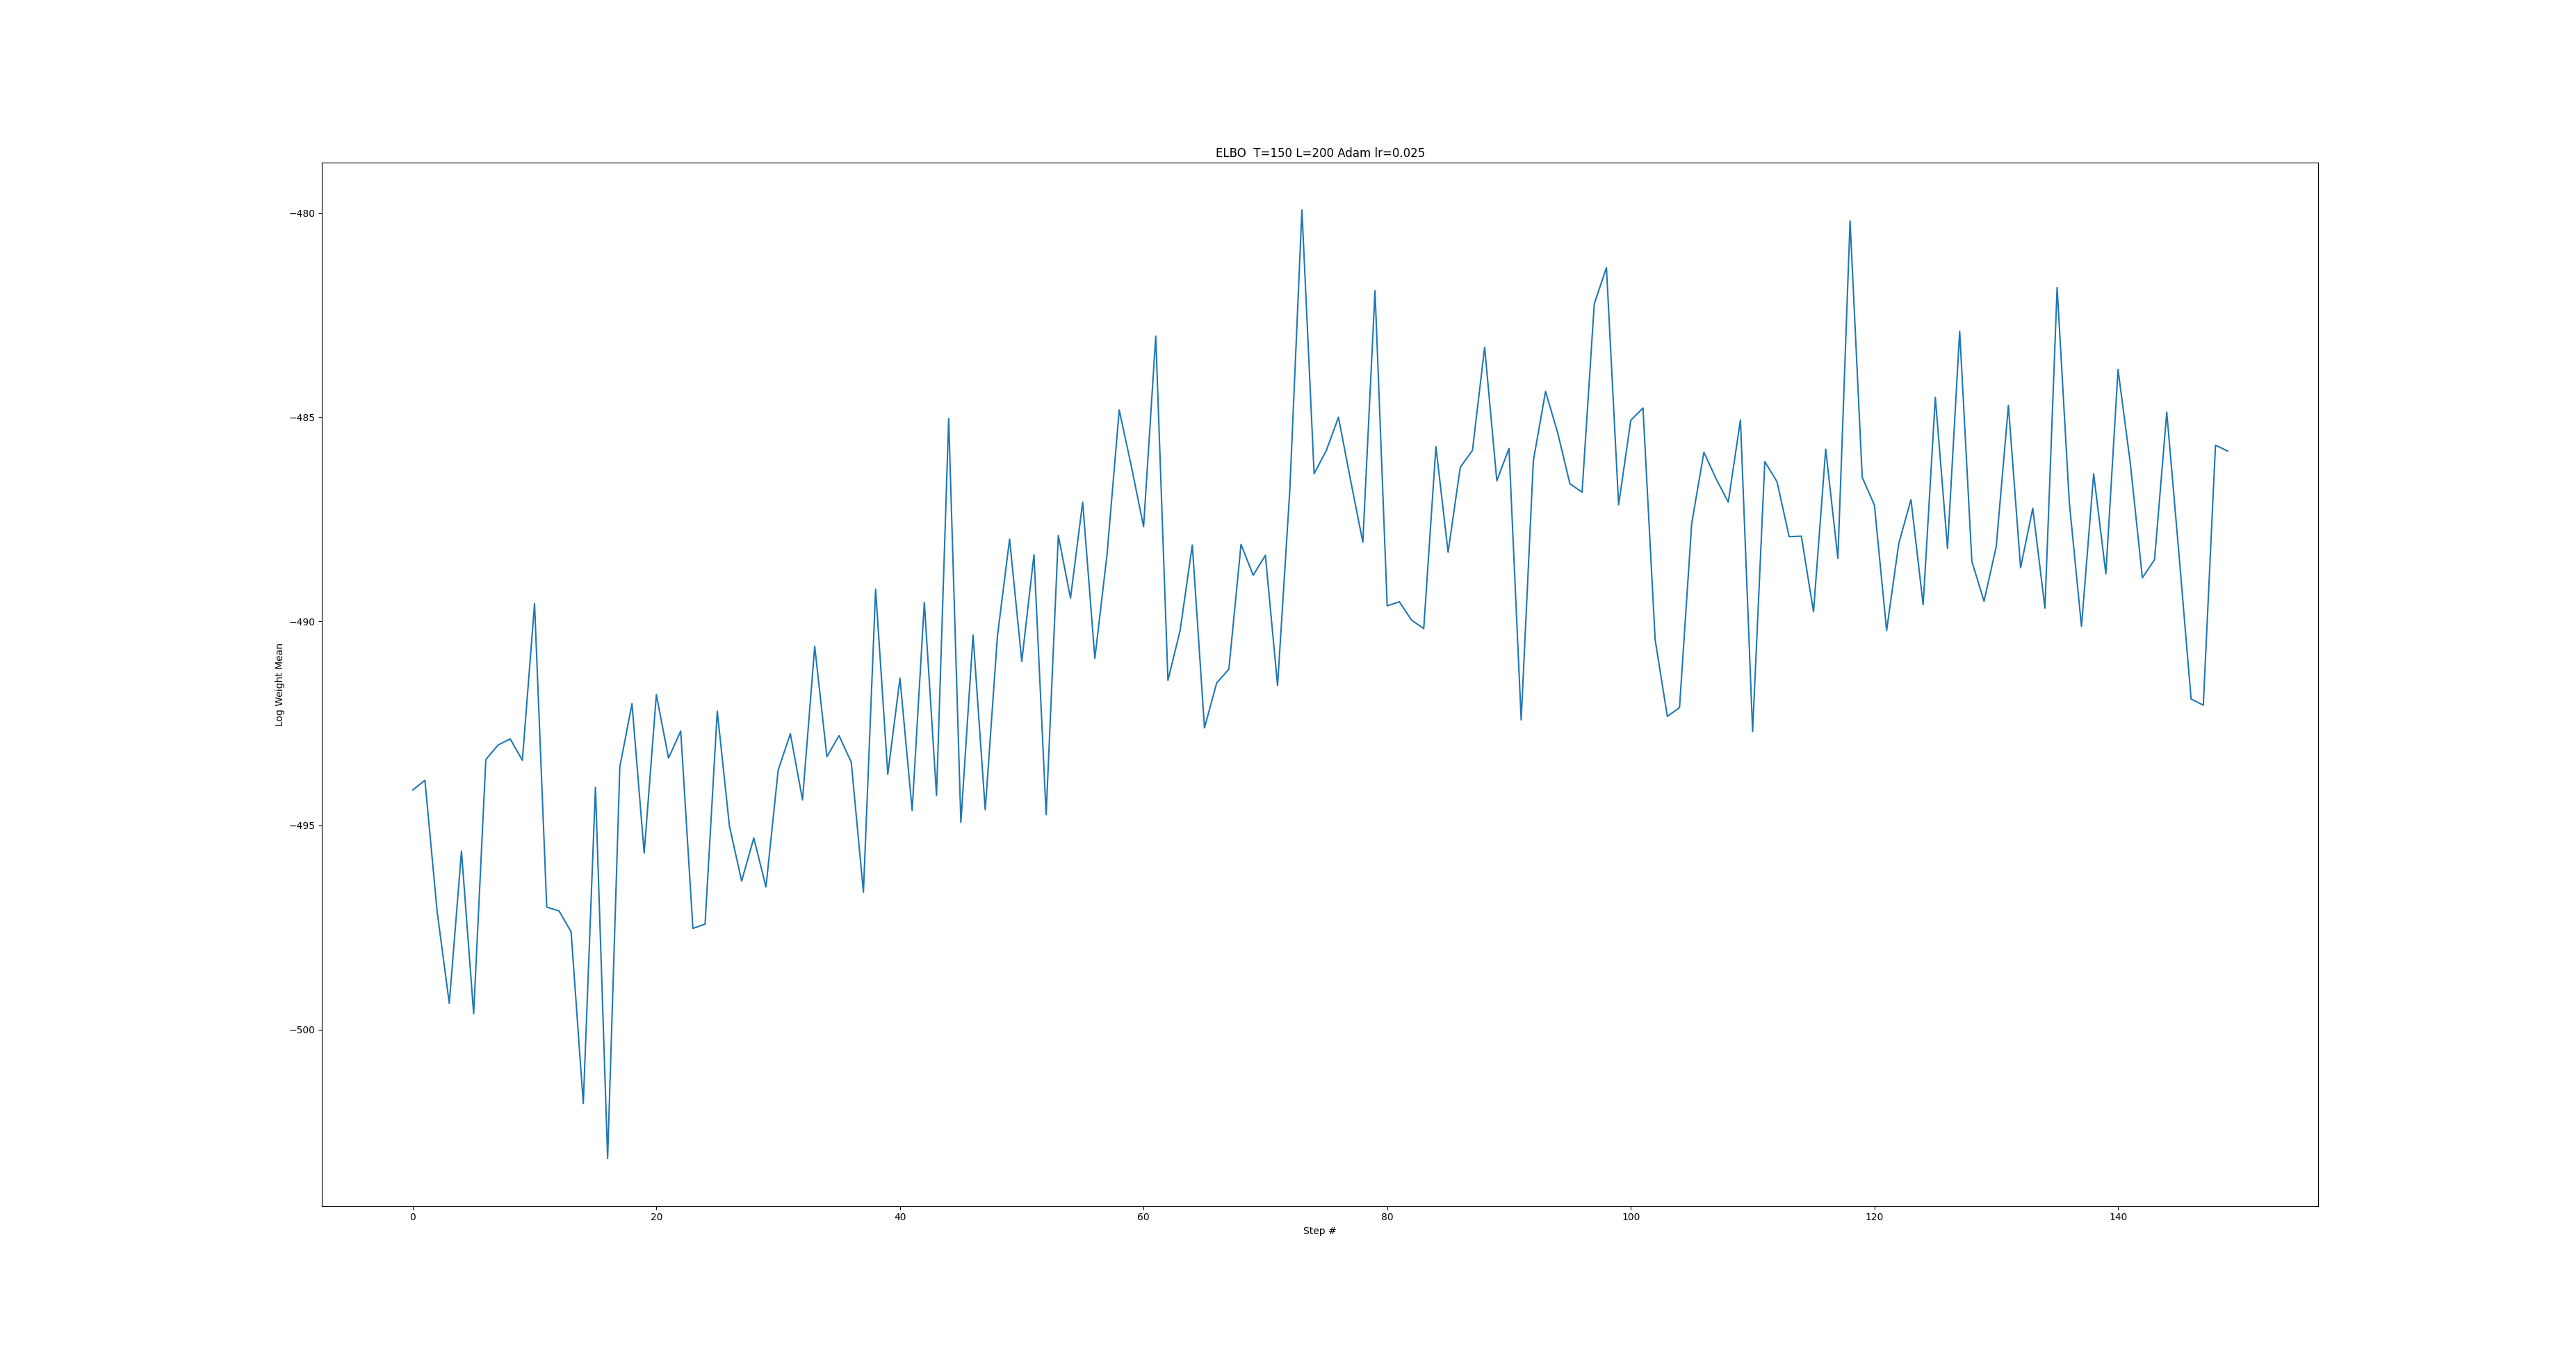
\includegraphics[width=\linewidth]{Figures/elbo_4Adam.png}
	\captionof{figure}{ELBO plot}
\end{center}
\begin{center}
	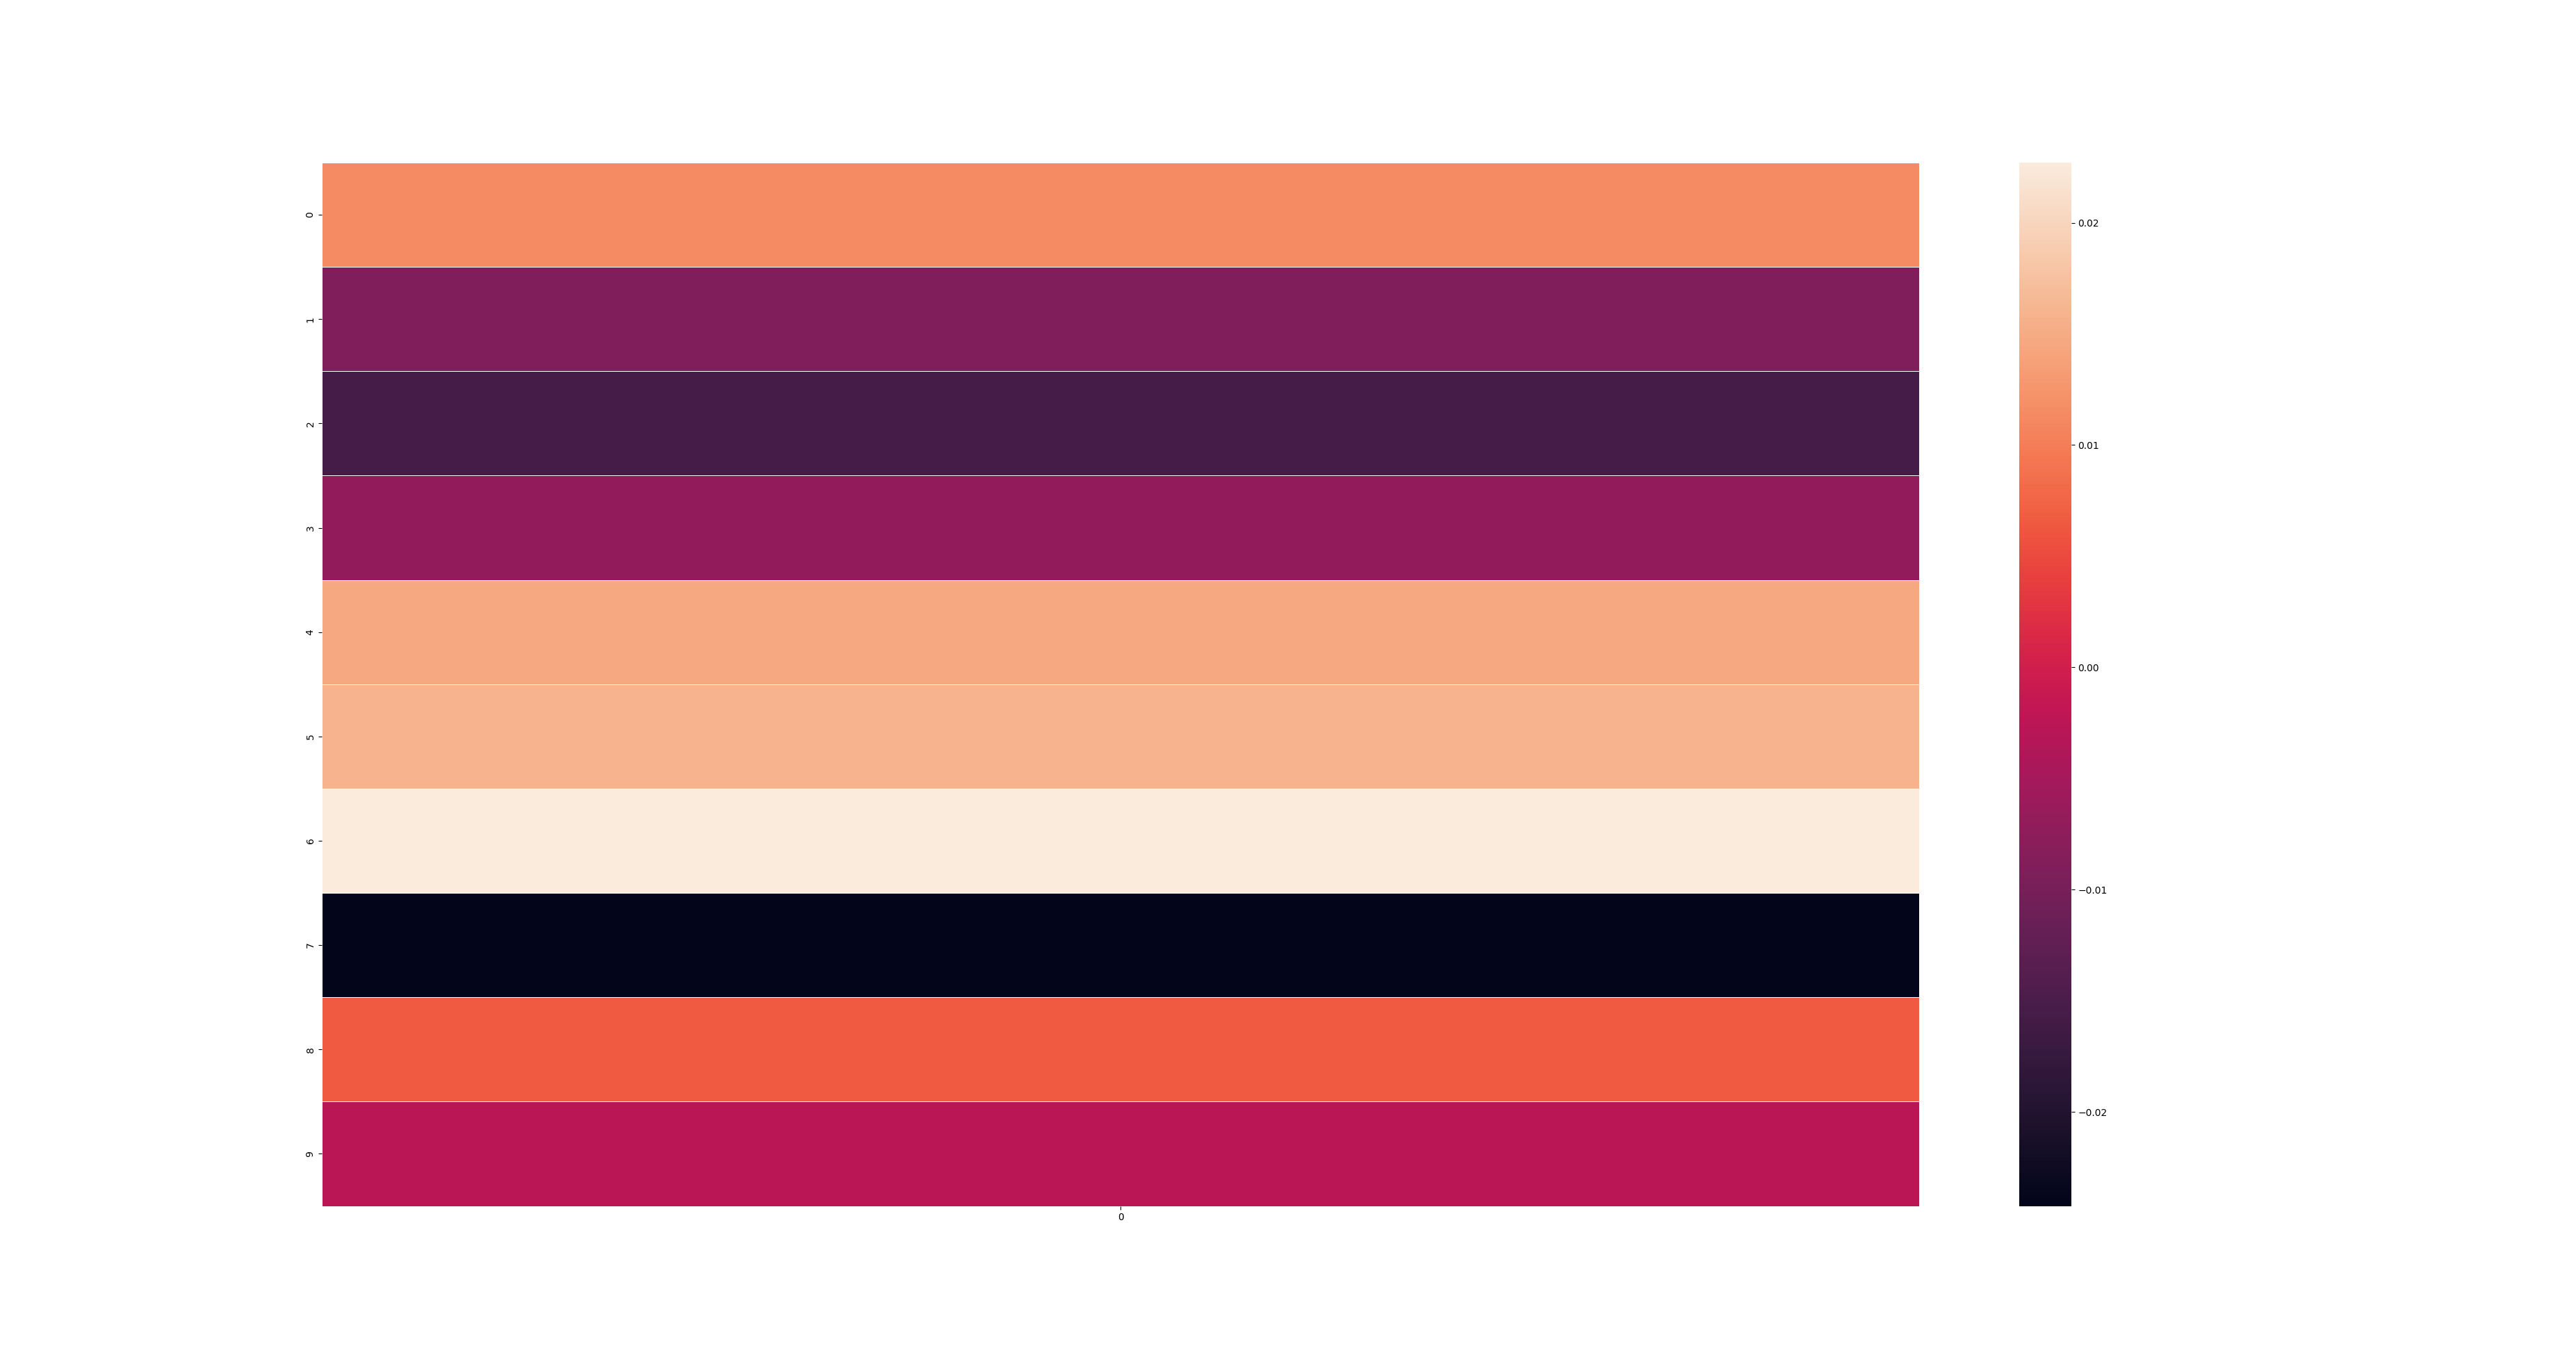
\includegraphics[width=\linewidth]{Figures/W0.png}
	\captionof{figure}{Heatmap of expectation of $W_0$}
\end{center}
\begin{center}
	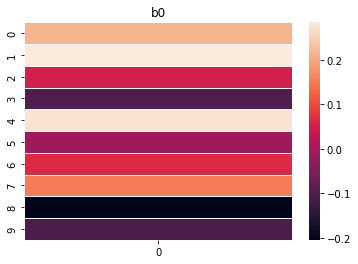
\includegraphics[width=\linewidth]{Figures/b0.png}
	\captionof{figure}{Heatmap of expectation of $b_0$}
\end{center}
\begin{center}
	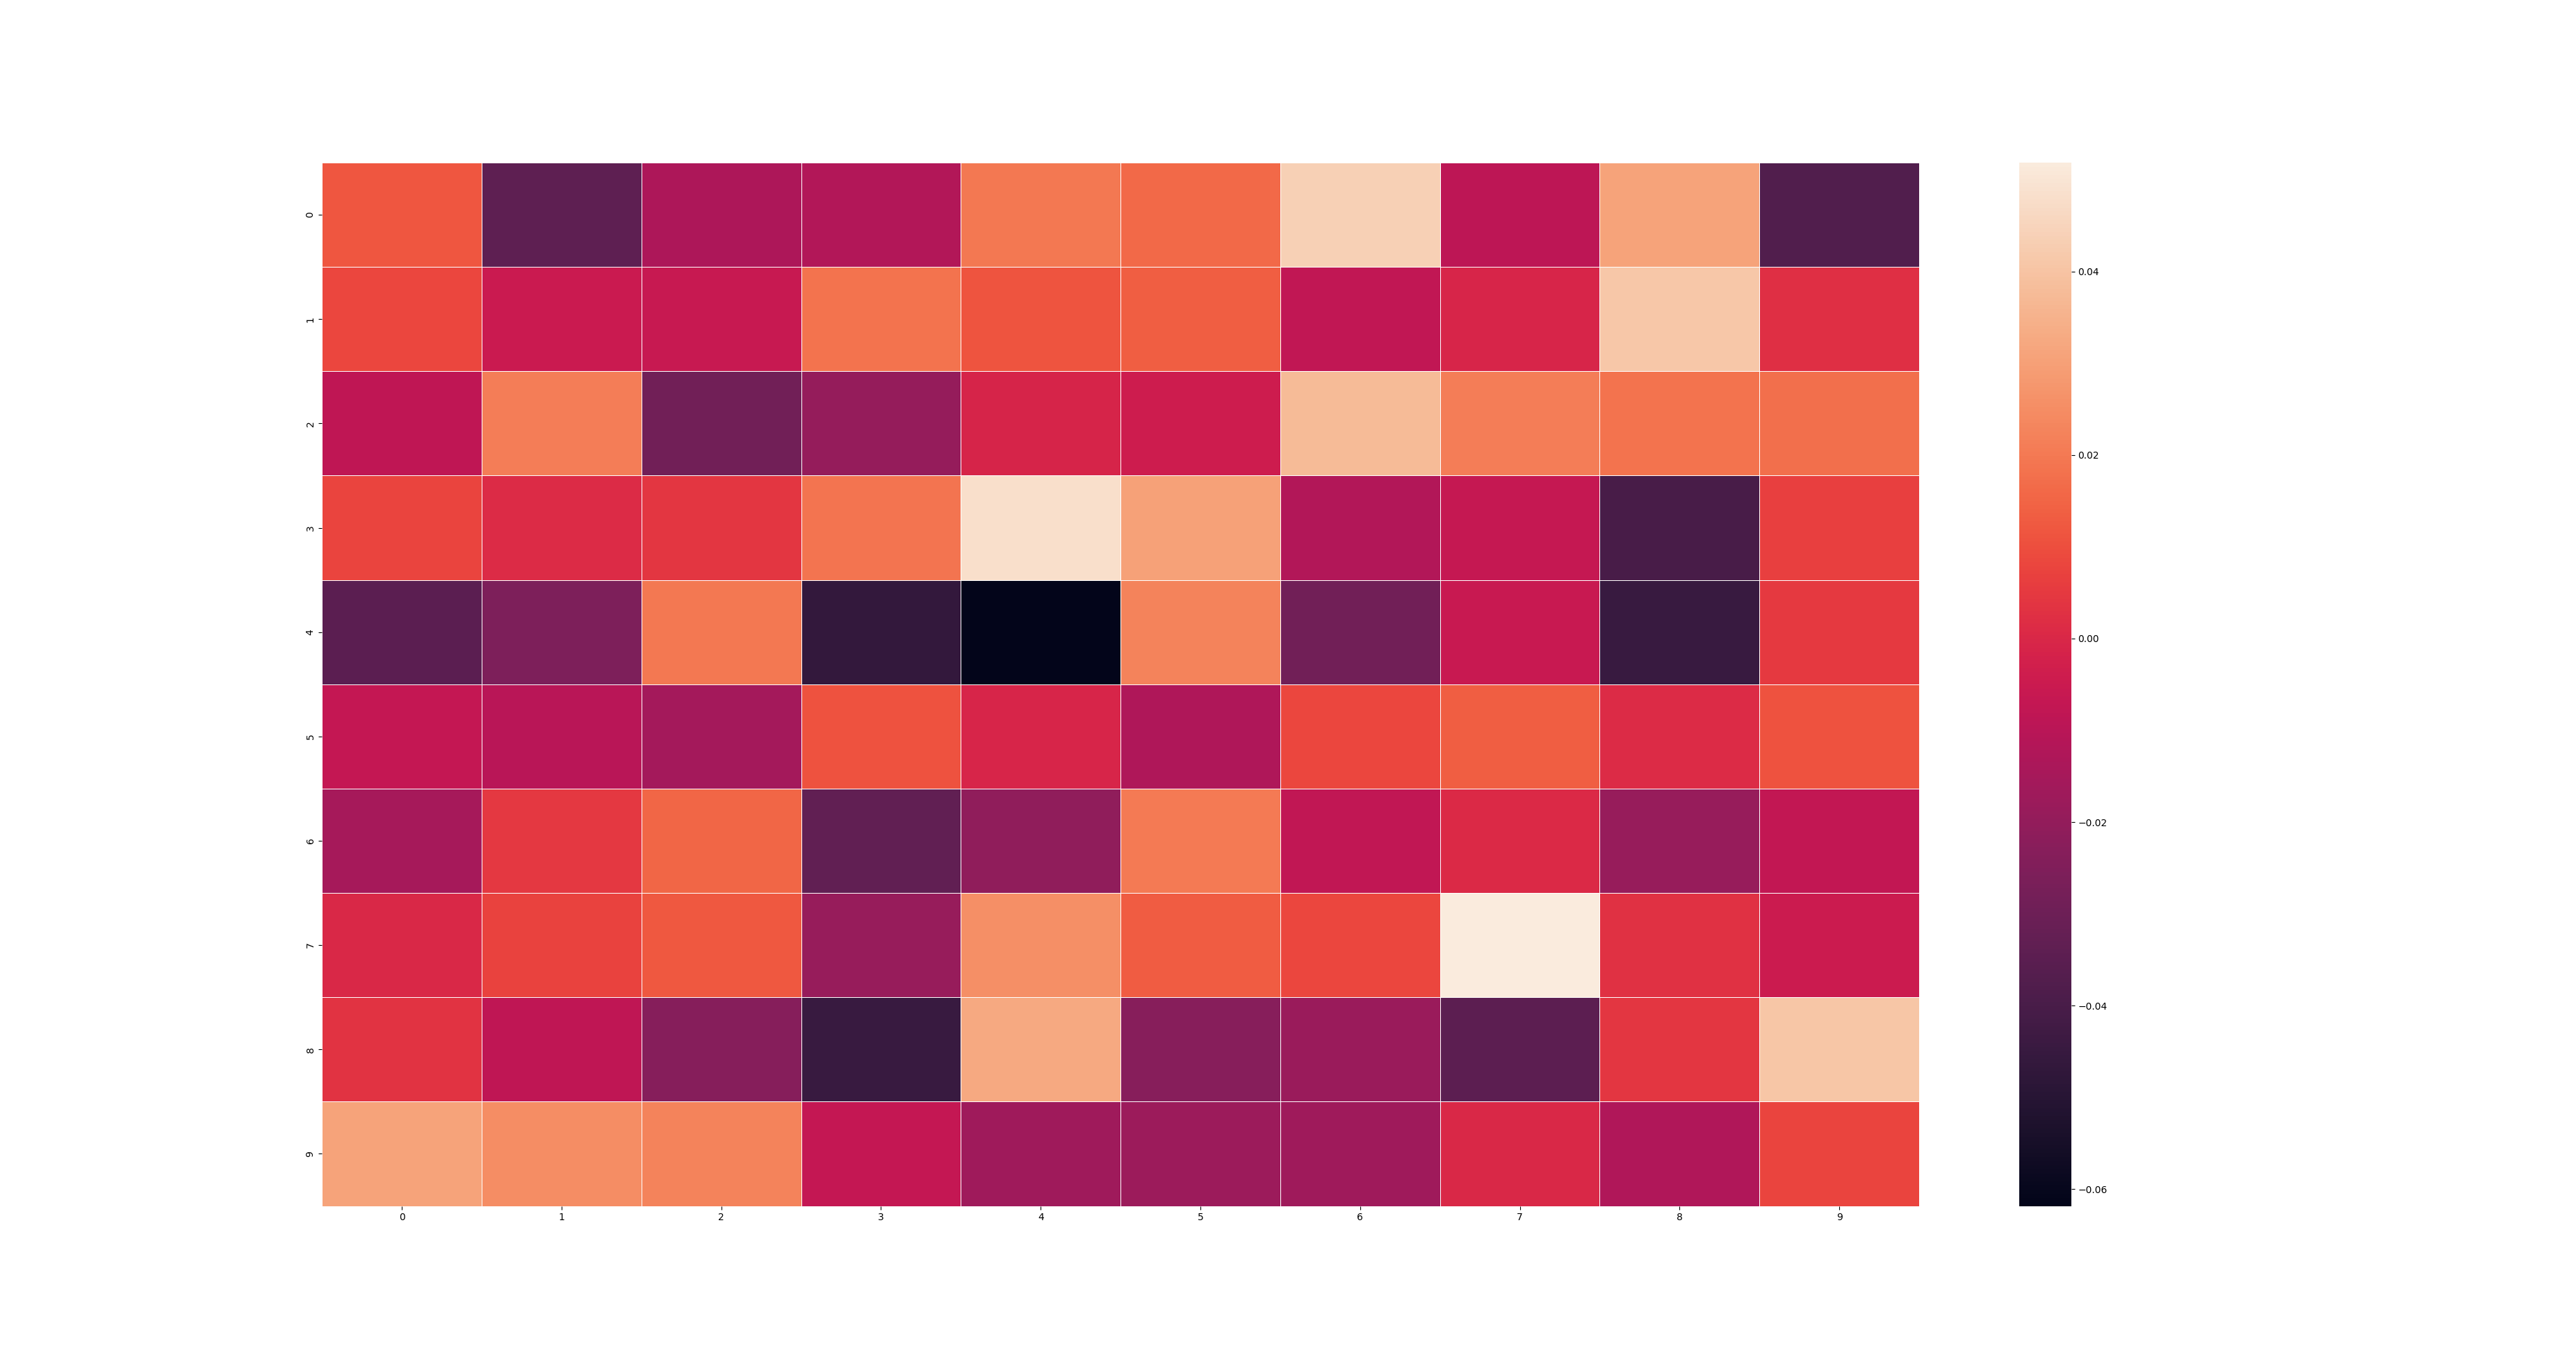
\includegraphics[width=\linewidth]{Figures/W1.png}
	\captionof{figure}{Heatmap of expectation of $W_1$}
\end{center}
\begin{center}
	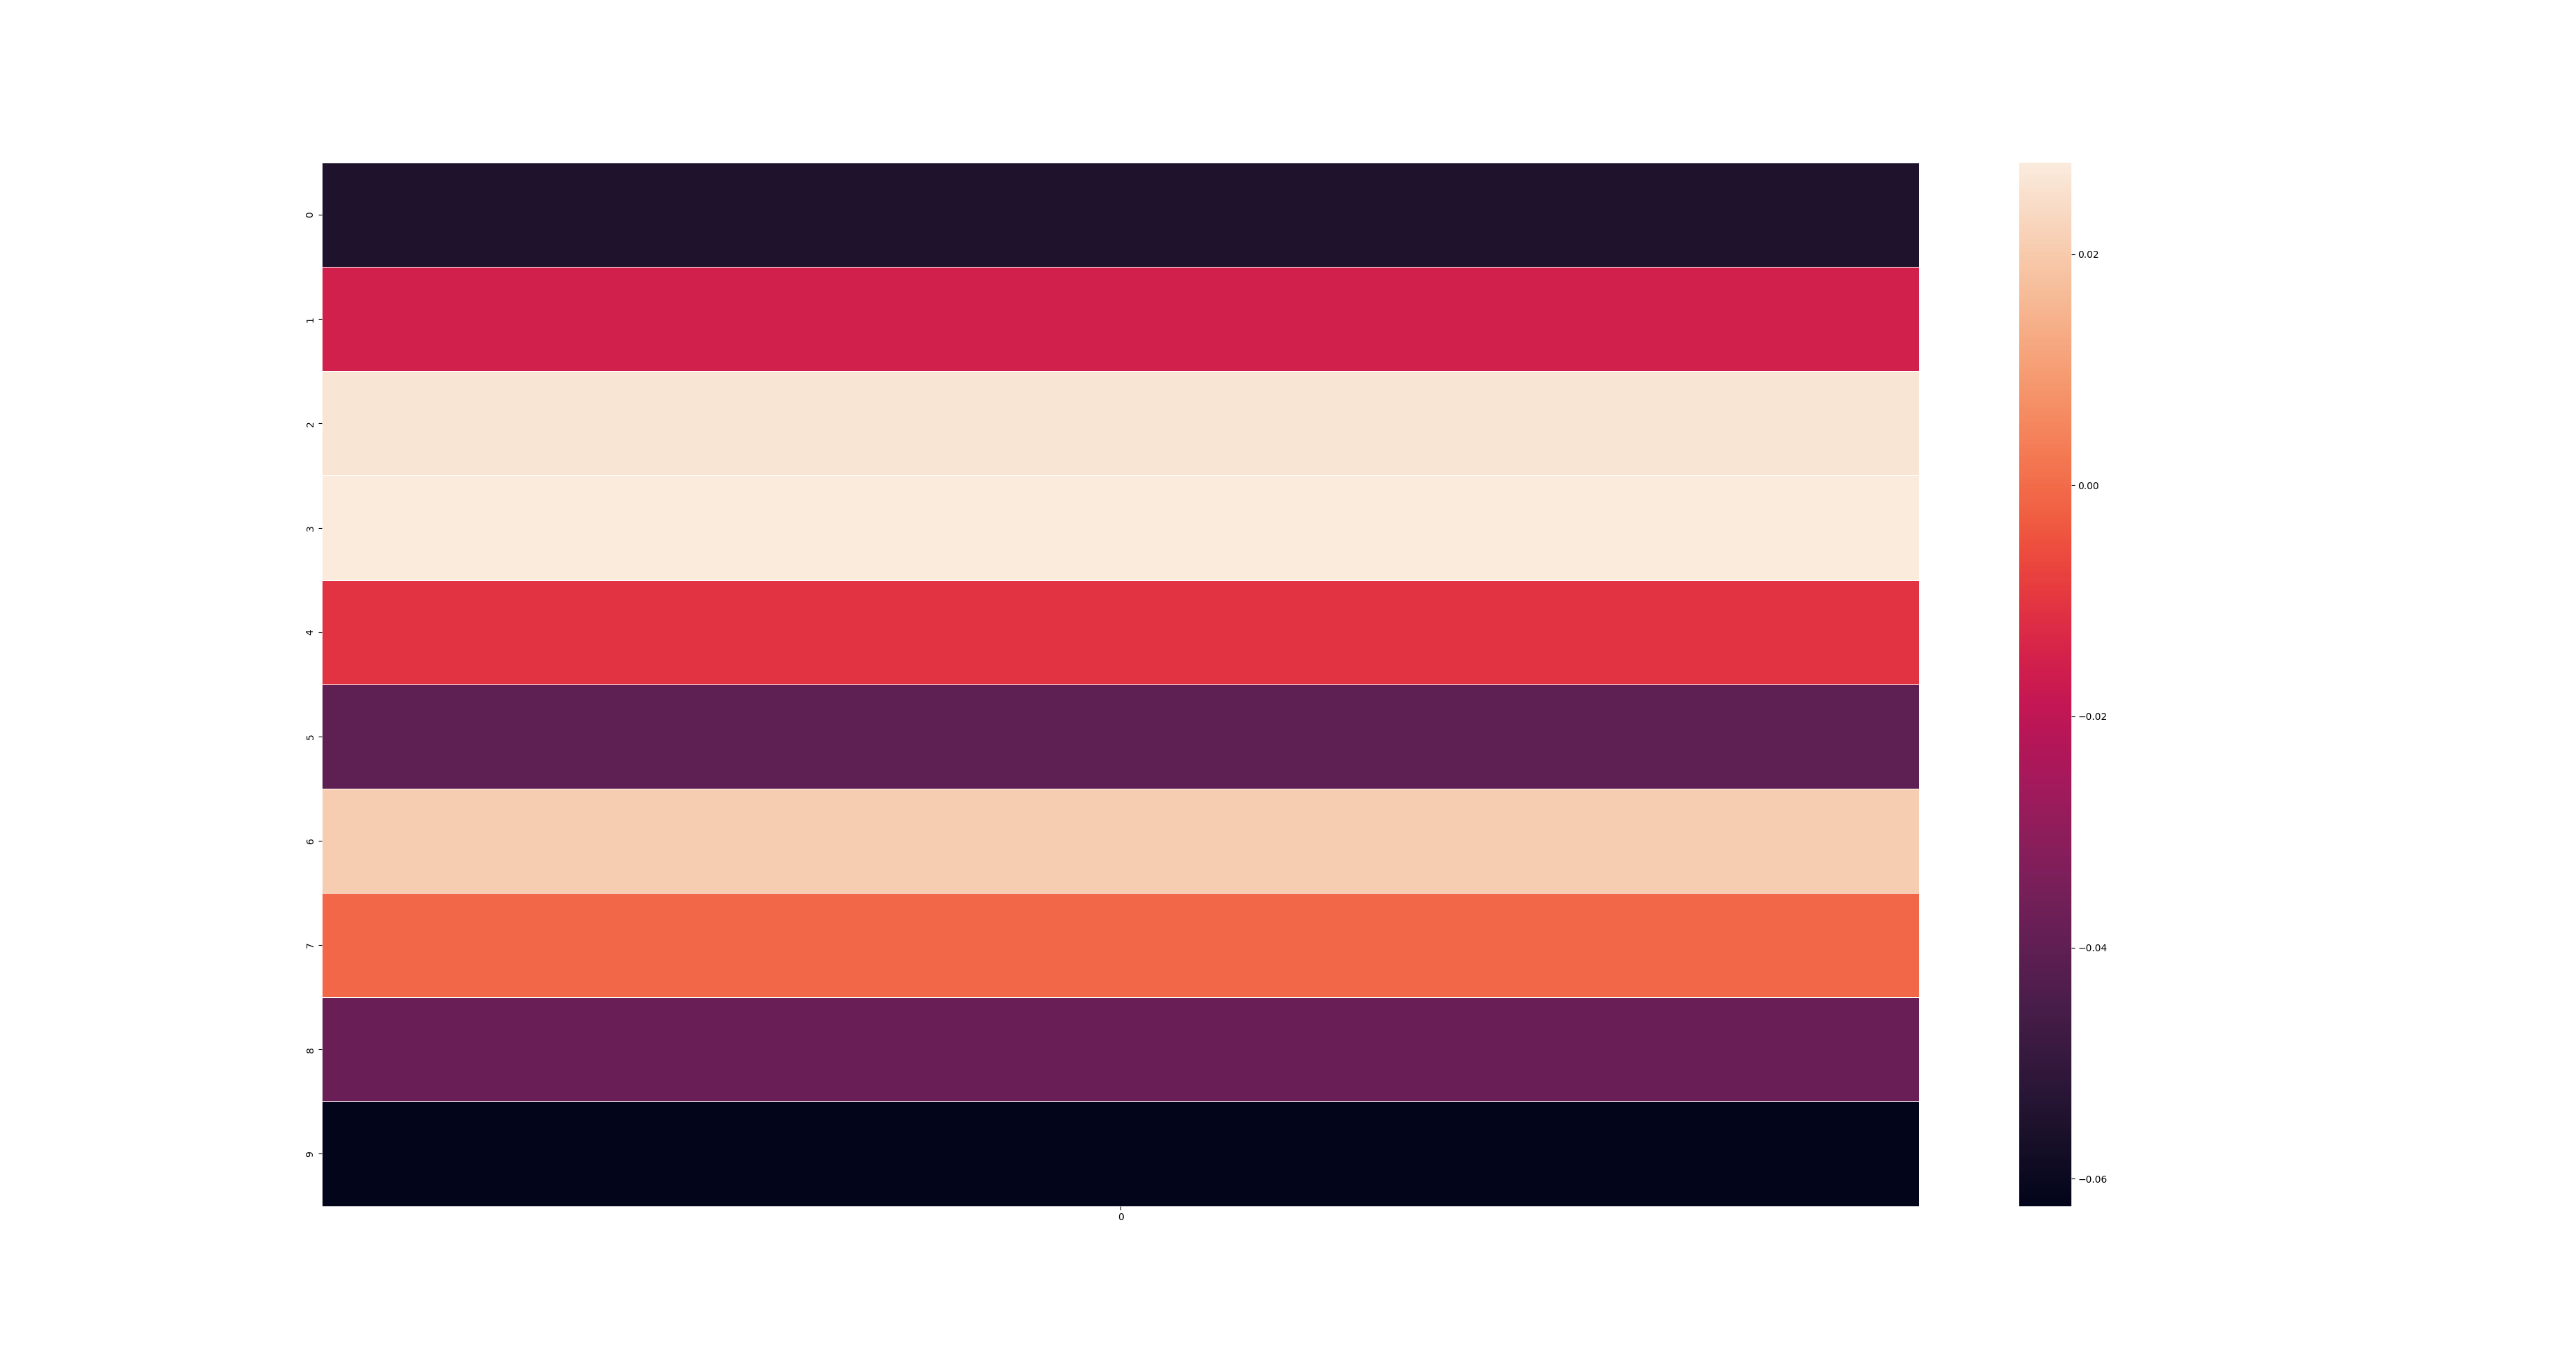
\includegraphics[width=\linewidth]{Figures/b1.png}
	\captionof{figure}{Heatmap of expectation of $b_1$}
\end{center}
Gradient descent optimization assumes a fix structure to the parameters of the network and adjust weights of the network. In BBVI we are learning the distribution that the parameters come from, i.e. once we know the distribution for the parameters of the network we can instantiate networks that are all supposed to solve the same problem. 
\subsection{Program 5}
For this program I am going to get creative about approximating the \emph{Uniform} distribution using $\tanh$ functions. I have used Wolfram Alpha to check some concrete examples, but a derivation to my approach:
\begin{equation}\begin{array}{rcl}
 f_{+}(x) &=& 0.5\tanh(x) + 0.5 \in [0,1] \\
 \lim_{x\rightarrow \infty} f_{+}(x) &=& 1 \\
 \lim_{x\rightarrow -\infty} f_{+}(x) &=& 0
\end{array}\end{equation}
If we define $f_{-}(x) = -0.5\tanh(x) + 0.5$, then $x\rightarrow \infty$ $f_{-}(x) =0$ and $x\rightarrow -\infty$ $f_{-}(x) = 1$. We can scale how fast the transition occurs with a parameter $s>0$ and translate where the transition occurs with $a$:
\begin{equation}\begin{array}{rcl}
 f(x) &=& 0.5\tanh(s(x-a)) + 0.5
\end{array}
\end{equation}
To approximate \texttt{Uniform(0,1)} we compose $f_{+}$ and $f_{-}$ as follows:
\begin{equation}\begin{array}{rcl}
\text{Uniform}(x)[0,1] &\approx& 0.5\left(\tanh(s(x)) - \tanh(s(x-1))\right)\\
\hat{\mathcal{U}}(x)[a,b] &=& \frac{1}{b-a}\left(0.5\left(\tanh(s(x+a)) - \tanh(s(x-b))\right)\right)
\end{array}\end{equation}
The question is the above a real probability density function? Using Wolfram Alpha and as an example $s = 10000$, $b = 1$ and $a = -1$ then $\int_{-\infty}^{\infty}\hat{\mathcal{U}}(x)[a,b]dx = 1$. Why use $\tanh$ functions? They are differentiable everywhere, as $s\rightarrow \infty$ the approximation gets closer and closer to the real distribution. However making $s$ large means the gradient vanishes very quickly when scored outside the support of the distribution. Thus picking $s$ to have smooth and non-zero derivatives outside the support is essential.

\begin{verbatim}
Collect samples denoted by program 5:
Elapsed time for program  5 .daphne is:  0:01:02.974768  seconds
Mean of samples:  tensor(6.5028)
and variance of samples:  tensor(1.0372)
{'sample1': Normal(loc: 0.3225950300693512, scale: 6.593713283538818), 'sample2': <distributions.Uniform object at 0x7f202702a3d0>}
\end{verbatim}
\begin{center}
	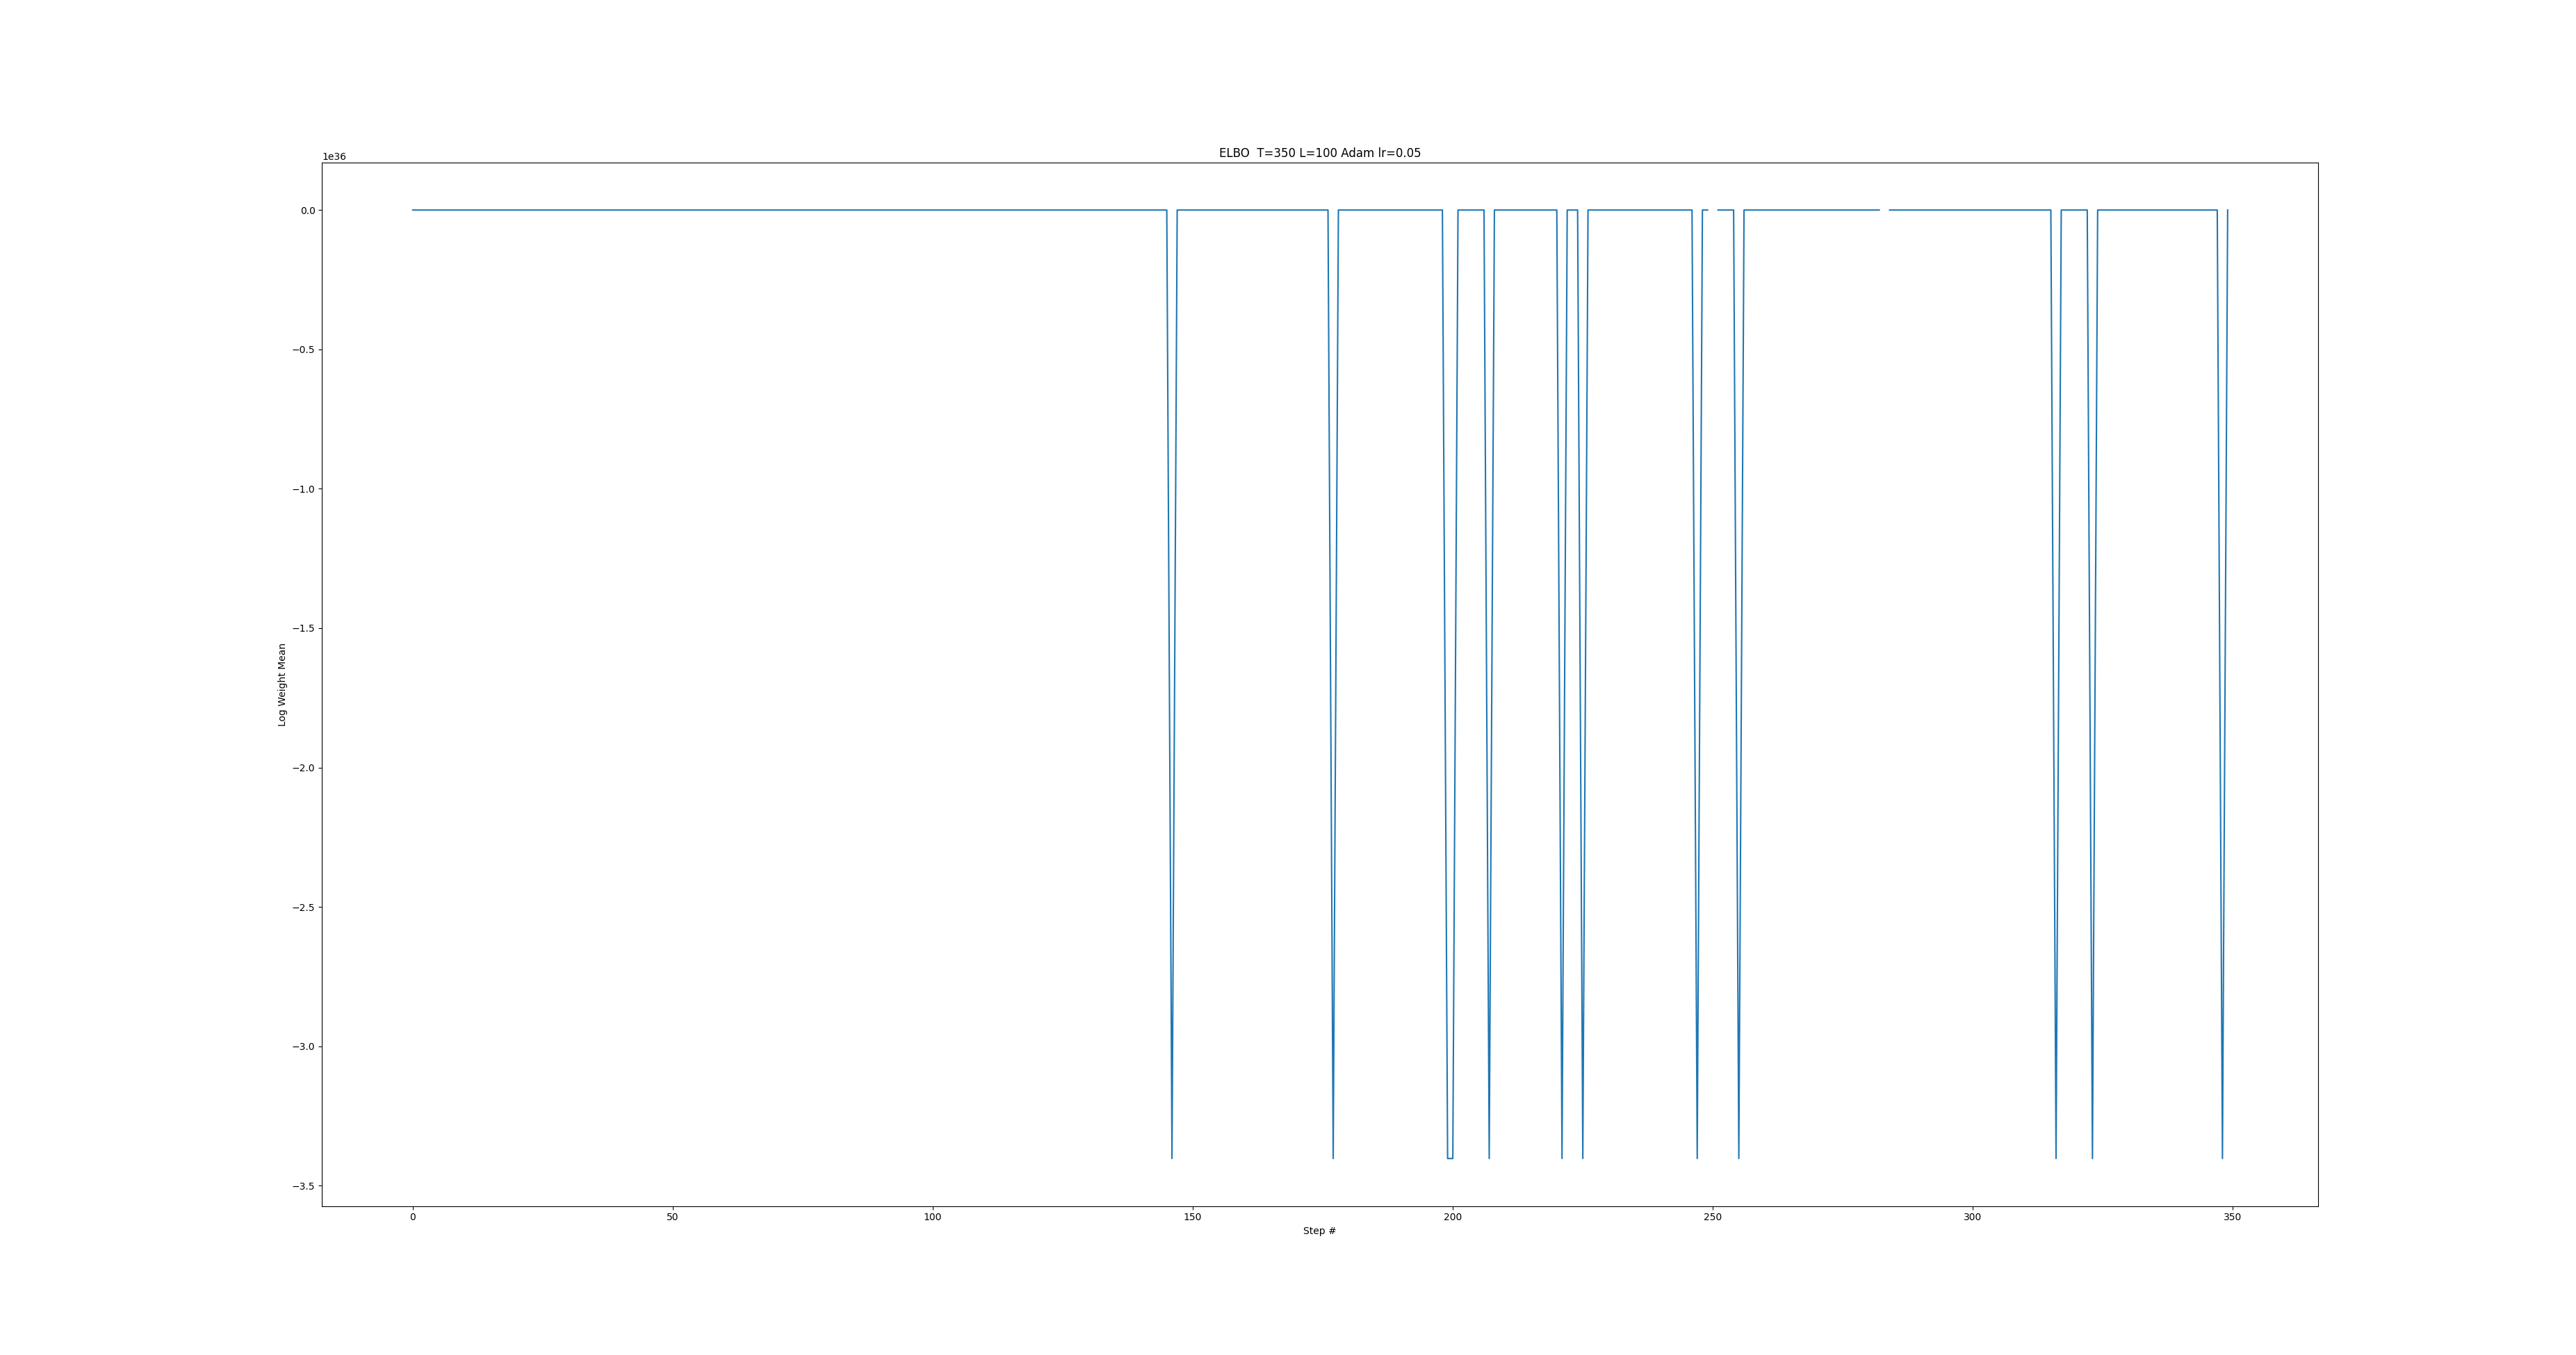
\includegraphics[width=\linewidth]{Figures/elbo_5Adam.png}
	\captionof{figure}{ELBO plot}
\end{center}
\begin{center}
	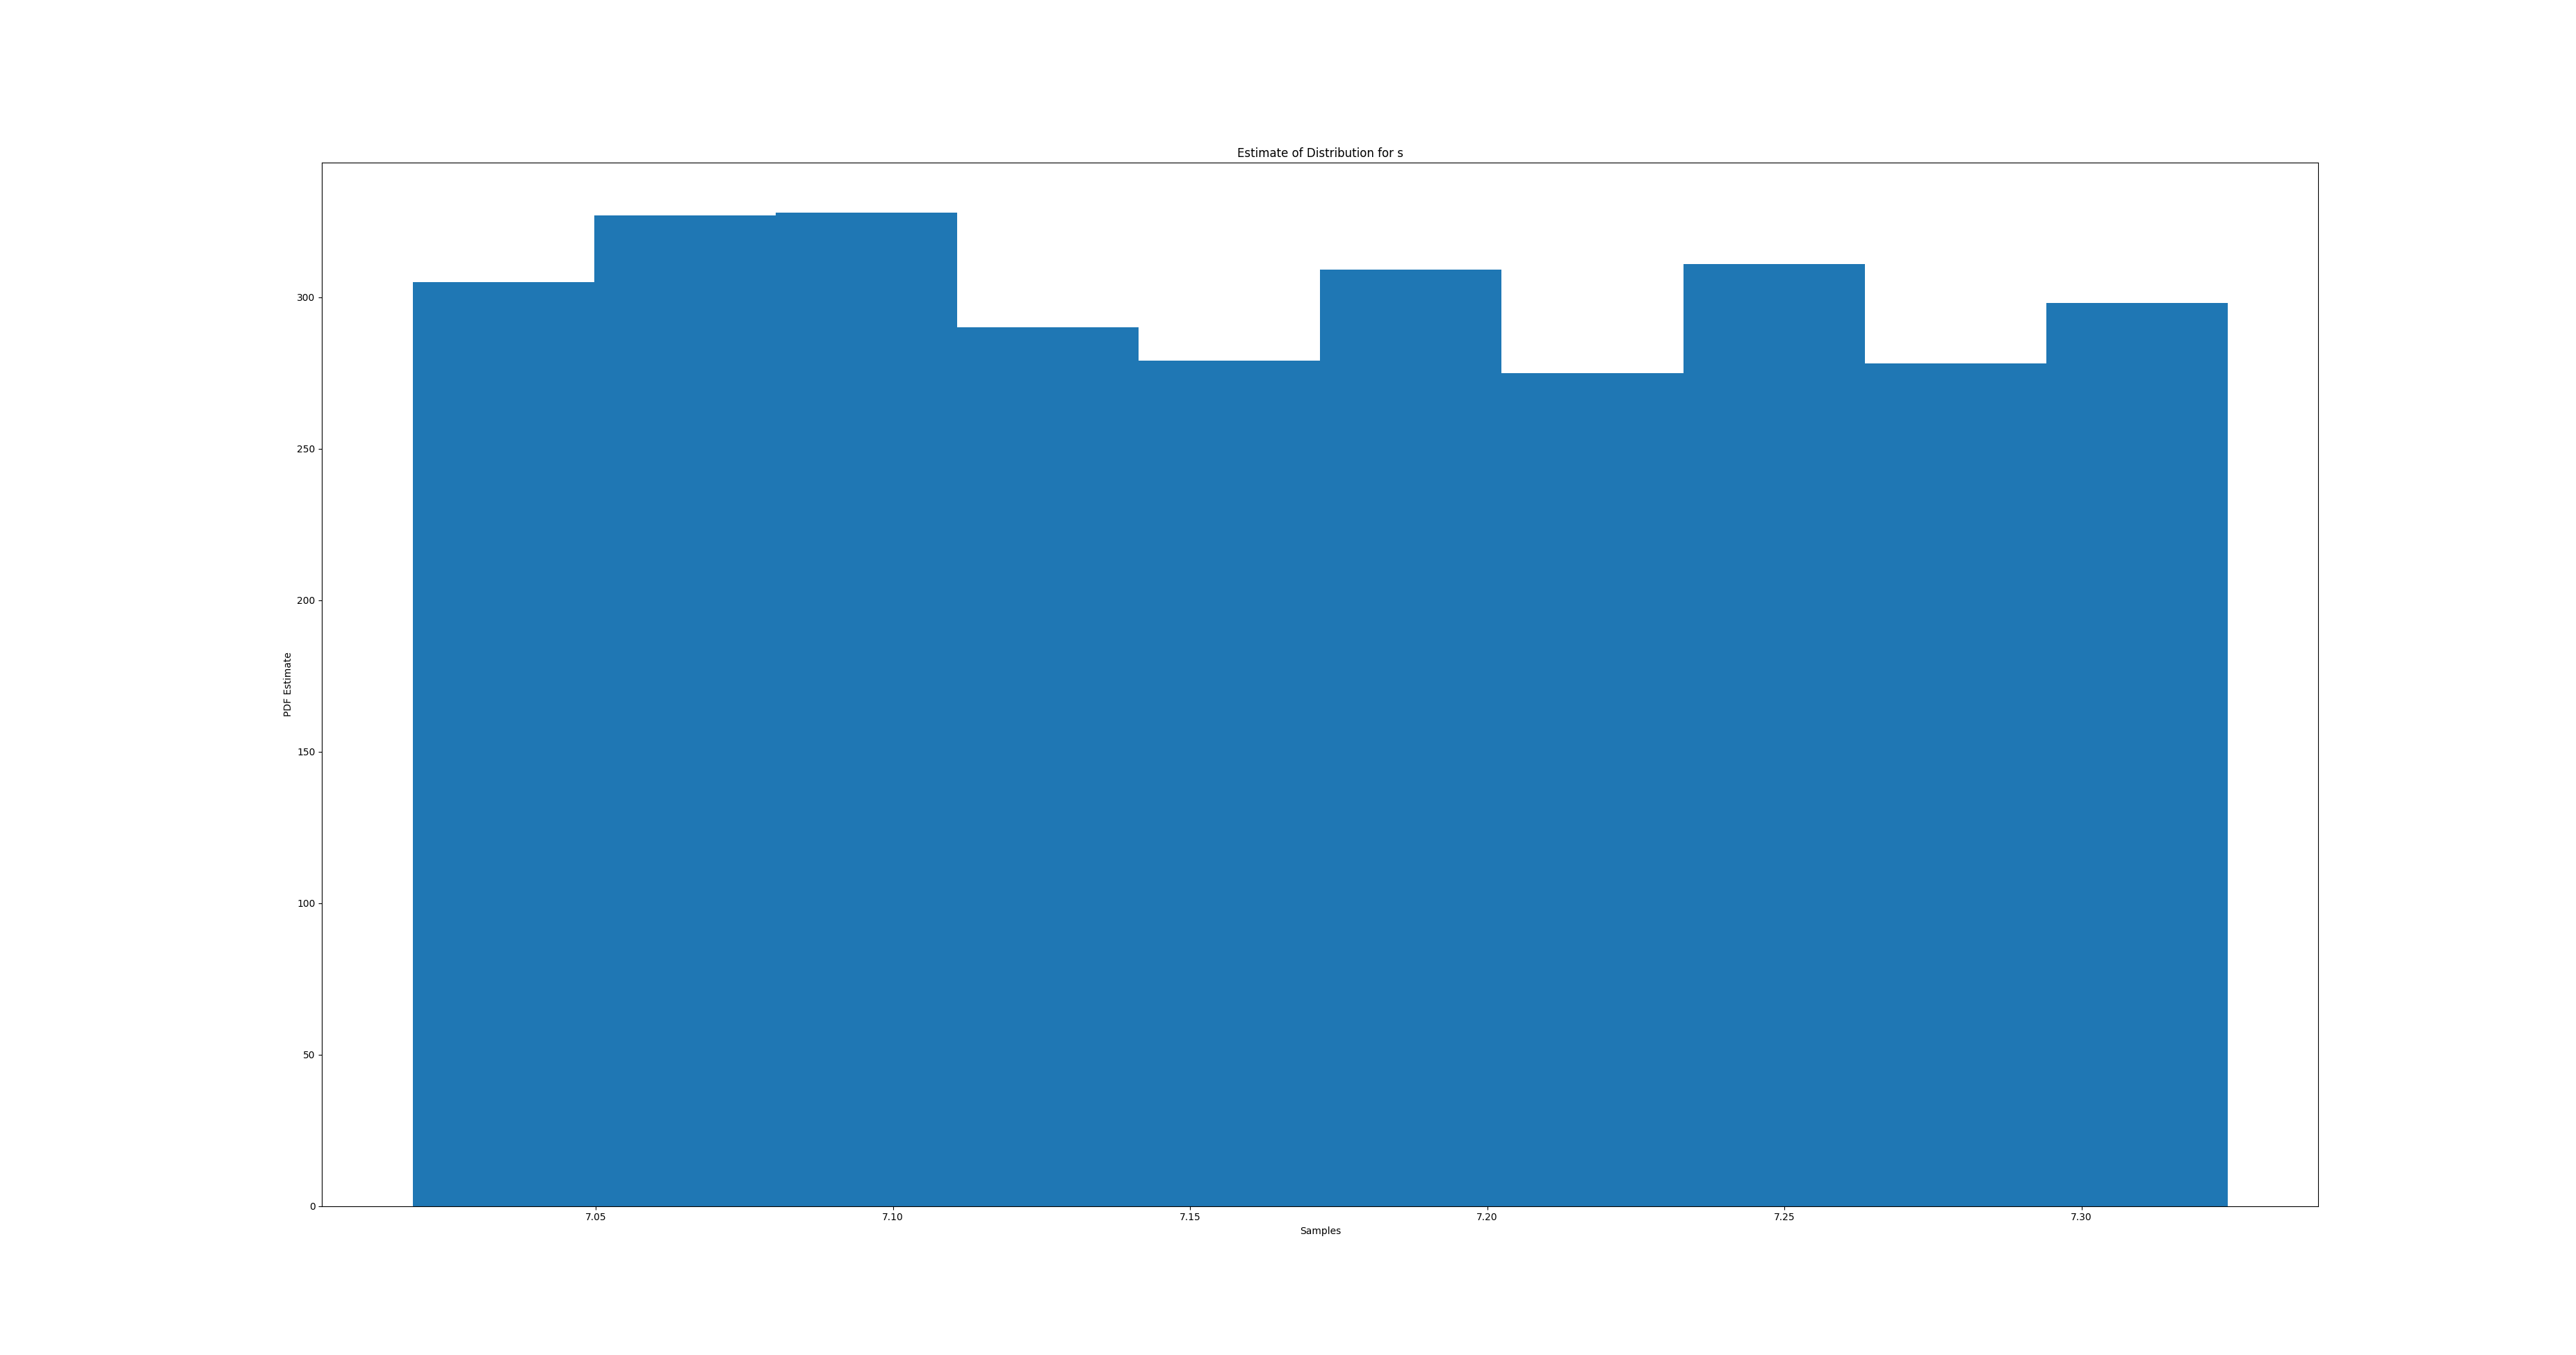
\includegraphics[width=\linewidth]{Figures/pdfEstP5.png}
	\captionof{figure}{Distribution Estimate for $s$ from $\mathcal{Q}$}
\end{center}
\begin{center}
	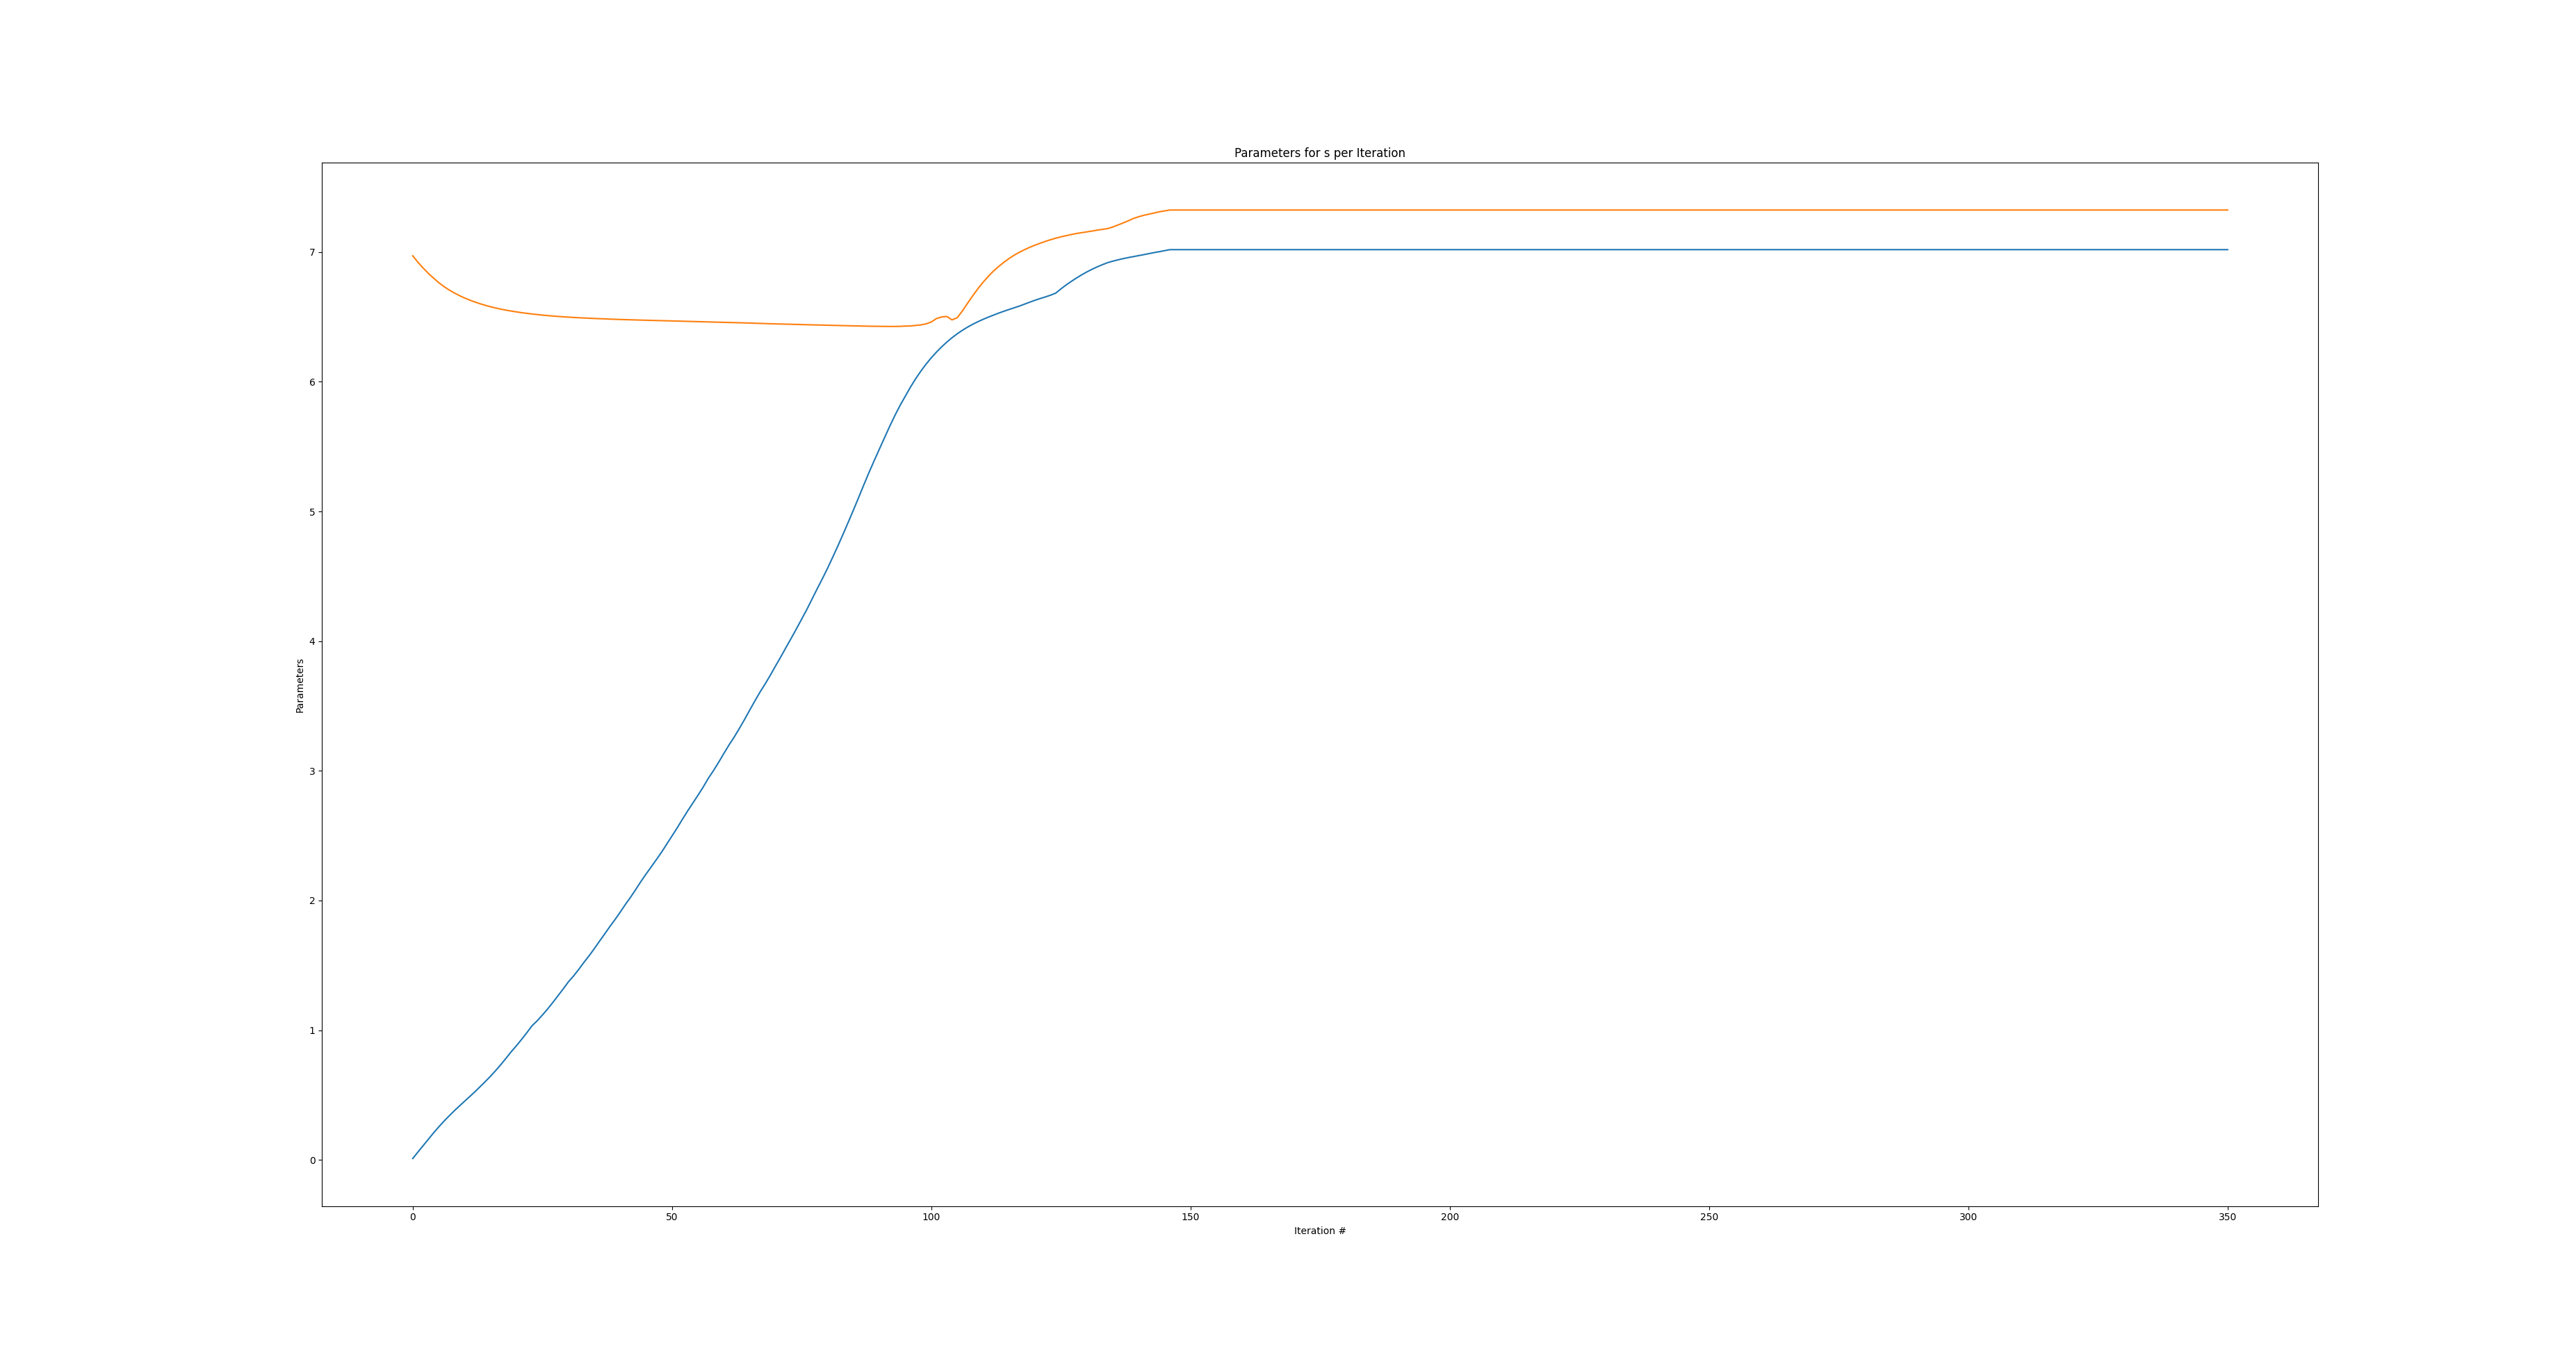
\includegraphics[width=\linewidth]{Figures/estParamsP5.png}
	\captionof{figure}{Parameters high and low for $\mathcal{Q}$ over iterations}
\end{center}

\end{document}
